%%%%%%%%%%%%%%%%%%%%%%%%%%%%%%%%%%%%%%%%%%%%%%%%%%%%%%%%%%%%%%%%%%%%%%%
%
%  A small sample UNSW Honours Thesis file.
%  Any questions to Ian Doust i.doust@unsw.edu.au
%
% Edited CSG 11.9.2015, use some of Gery's ideas for front matter; add a conclusion chapter.
%%%%%%%%%%%%%%%%%%%%%%%%%%%%%%%%%%%%%%%%%%%%%%%%%%%%%%%%%%%%%%%%%%%%%%%
%
%  The first part pulls in a UNSW Thesis class file.  This one is
%  slightly nonstandard and has been set up to do a couple of
%  things automatically
%
 
\documentclass[honours,12pt]{unswthesis}
\linespread{1.3}
\usepackage{kotex}
\usepackage{amsfonts}
\usepackage{amssymb}
\usepackage{amsthm}
\usepackage{latexsym,amsmath}
\usepackage{graphicx}
\usepackage{pgfplots}
\usepackage{afterpage}
\usepackage[ ]{algorithm2e}
\usepackage{bm}
\usepackage{tikz}
\usetikzlibrary{bayesnet}
\usepackage{boondox-cal}
\usepackage{cite}
\allowdisplaybreaks[1]
%%%%%%%%%%%%%%%%%%%%%%%%%%%%%%%%%%%%%%%%%%%%%%%%%%%%%%%%%%%%%%%%%
%
%  The following are some simple LaTeX macros to give some
%  commonly used letters in funny fonts. You may need more or less of
%  these
%
\newcommand{\R}{\mathbb{R}}
\newcommand{\Q}{\mathbb{Q}}
\newcommand{\C}{\mathbb{C}}
\newcommand{\N}{\mathbb{N}}
\newcommand{\F}{\mathbb{F}}
\newcommand{\PP}{\mathbb{P}}
\newcommand{\T}{\mathbb{T}}
\newcommand{\Z}{\mathbb{Z}}
\newcommand{\B}{\mathfrak{B}}
\newcommand{\BB}{\mathcal{B}}
\newcommand{\M}{\mathfrak{M}}
\newcommand{\X}{\mathfrak{X}}
\newcommand{\Y}{\mathfrak{Y}}
\newcommand{\CC}{\mathcal{C}}
\newcommand{\E}{\mathbb{E}}
\newcommand{\cP}{\mathcal{P}}
\newcommand{\cS}{\mathcal{S}}
\newcommand{\A}{\mathcal{A}}
\newcommand{\ZZ}{\mathcal{Z}}
%%%%%%%%%%%%%%%%%%%%%%%%%%%%%%%%%%%%%%%%%%%%%%%%%%%%%%%%%%%%%%%%%%%%%
%
% The following are much more esoteric commands that I have left in
% so that this file still processes. Use or delete as you see fit
%
\newcommand{\var}{\mathop{\rm var}}
\newcommand{\Var}{\mathrm{Var}}
\newcommand{\ltp}{\mathrel{{\prec}_p}}
\newcommand{\lep}{\mathrel{{\preceq}_p}}
\def\brack#1{\left \{ #1 \right \}}
\def\bul{$\bullet$\ }
\def\cl{{\rm cl}}
\let\del=\partial
\def\enditem{\par\smallskip\noindent}
\def\implies{\Rightarrow}
\def\inpr#1,#2{\t \hbox{\langle #1 , #2 \rangle} \t}
\def\ip<#1,#2>{\langle #1,#2 \rangle}
\def\lp{\ell^p}
\def\maxb#1{\max \brack{#1}}
\def\minb#1{\min \brack{#1}}
\def\mod#1{\left \vert #1 \right \vert}
\def\norm#1{\left \Vert #1 \right \Vert}
\def\paren(#1){\left( #1 \right)}
\def\qed{\hfill \hbox{$\Box$} \smallskip}
\def\sbrack#1{\Bigl \{ #1 \Bigr \} }
\def\ssbrack#1{ \{ #1 \} }
\def\smod#1{\Bigl \vert #1 \Bigr \vert}
\def\smmod#1{\bigl \vert #1 \bigr \vert}
\def\ssmod#1{\vert #1 \vert}
\def\sspmod#1{\vert\, #1 \, \vert}
\def\snorm#1{\Bigl \Vert #1 \Bigr \Vert}
\def\ssnorm#1{\Vert #1 \Vert}
\def\sparen(#1){\Bigl ( #1 \Bigr )}
\DeclareMathOperator*{\argmin}{arg\,min}
\DeclareMathOperator*{\argmax}{arg\,max}
\newcommand\blankpage{%
    \null
    \thispagestyle{empty}%
    \addtocounter{page}{-1}%
    \newpage}

%%%%%%%%%%%%%%%%%%%%%%%%%%%%%%%%%%%%%%%%%%%%%%%%%%%%%%%%%%%%%%
%
% These environments allow you to get nice numbered headings
%  for your Theorems, Definitions etc.  
%
%  Environments
%
%%%%%%%%%%%%%%%%%%%%%%%%%%%%%%%

\newtheorem{theorem}{Theorem}[section]
\newtheorem{lemma}[theorem]{Lemma}
\newtheorem{proposition}[theorem]{Proposition}
\newtheorem{corollary}[theorem]{Corollary}
\newtheorem{conjecture}[theorem]{Conjecture}

\newtheorem{remark}[theorem]{Remark}
\newtheorem{question}[theorem]{Question}
\newtheorem{notation}[theorem]{Notation}
\numberwithin{equation}{section}
\theoremstyle{definition}
\newtheorem{definition}[theorem]{Definition}
\newtheorem{example}[theorem]{Example}
%%%%%%%%%%%%%%%%%%%%%%%%%%%%%%%%%%%%%%%%%%%%%%%%%%%%%%%%%%%%%%%%%%
%
%  If you've got some funny special words that LaTeX might not
% hyphenate properly, you can give it a helping hand:
%
\hyphenation{Mar-cin-kie-wicz Rade-macher}

%%%%%%%%%%%%%%%%%%%%%%%%%%%%%%%%%%%%%%%%%%%%%%%%%%%%%%%%%%%%%%%%%%
% 
% OK...Now we get to some actual input.  The first part sets up
% the title etc that will appear on the front page
%
%%%%%%%%%%%%%%%%%%%%%%%%%%%%%%%%%%%%%%%%%%%%%%%%%%%%%%%%%%%%%%%%%

\title{Density Ratio Estimators for Variational Methods in Bayesian Neural Networks}

\authornameonly{Alexander Lam}

\author{\Authornameonly\\{\bigskip}Supervisor: Professor Scott Sisson}

\copyrightfalse
\figurespagefalse
\tablespagefalse

%%%%%%%%%%%%%%%%%%%%%%%%%%%%%%%%%%%%%%%%%%%%%%%%%%%%%%%%%%%%%%%%%
%
%  And now the document begins
%  The \beforepreface and \afterpreface commands puts the
%  contents page etc in
%
%%%%%%%%%%%%%%%%%%%%%%%%%%%%%%%%%%%%%%%%%%%%%%%%%%%%%%%%%%%%%%%%%%

\begin{document}

\beforepreface

\afterpage{\blankpage}

% plagiarism

\prefacesection{Plagiarism statement}

\vskip 10pc \noindent I declare that this thesis is my
own work, except where acknowledged, and has not been submitted for
academic credit elsewhere. 

\vskip 2pc  \noindent I acknowledge that the assessor of this
thesis may, for the purpose of assessing it:
\begin{itemize}
\item Reproduce it and provide a copy to another member of the University; and/or,
\item Communicate a copy of it to a plagiarism checking service (which may then retain a copy of it on its database for the purpose of future plagiarism checking).
\end{itemize}

\vskip 2pc \noindent I certify that I have read and understood the University Rules in
respect of Student Academic Misconduct, and am aware of any potential plagiarism penalties which may 
apply.\vspace{24pt}

\vskip 2pc \noindent By signing 
this declaration I am
agreeing to the statements and conditions above.
\vskip 2pc \noindent
Signed: \rule{7cm}{0.25pt} \hfill Date: \rule{4cm}{0.25pt} \newline
\vskip 1pc

\afterpage{\blankpage}

% Acknowledgements are optional


\prefacesection{Acknowledgements}

{\bigskip}Scott Sisson, Edwin Bonilla, Louis Tiao

{\bigskip\noindent}Trevor Trotman

{\bigskip\noindent}Honours Room Inhabitants, esp. Bouldering crew

{\bigskip\noindent}Discord Group+Kong+Brian

{\bigskip\noindent}Sunchit

{\bigskip\noindent}누나

{\bigskip\noindent}Family

{\bigskip\bigskip\bigskip\noindent} Lammy, 11 September 2018.

\afterpage{\blankpage}

% Abstract

\prefacesection{Abstract}
Never use ReLU output to estimate density ratios.\\
Class probability estimator = good, direct density ratio and direct log density ratio estimators = bad.\\ 
Also KL Divergence $>$ "CPE" Divergence for formulating estimator loss function but we already know that (although everyone seems to continue to use CPE divergence).
\afterpage{\blankpage}


\afterpreface

%%%%%%%%%%%%%%%%%%%%%%%%%%%%%%%%%%%%%%%%%%%%%%%%%%%%%%%%%%%%%%%%%%
%
% Now we can start on the first chapter
% Within chapters we have sections, subsections and so forth
%
%%%%%%%%%%%%%%%%%%%%%%%%%%%%%%%%%%%%%%%%%%%%%%%%%%%%%%%%%%%%%%%%%%

\afterpage{\blankpage}

\chapter{Introduction}\label{s-intro}


\section{Problem Context}
In machine learning, particularly for high dimensional applications such as image analysis, it is often desirable to build generative models, so that we can represent the data in lower dimensions via representation learning, and generate new data similar to the examples in our dataset. Assume our dataset $X=\{x^{(i)}\}^N_{i=1}\sim q^*(x)$ is $N$ i.i.d. samples of random variables $x$. Also assume $x$ can be generated by a stochastic process from a latent continuous random variable $z$. These models involve a posterior distribution $p(z|x)$ that maps the dataset $x$ to lower dimensional latent prior $z$ (e.g. $z\sim N(\mu,\Sigma)$) then simulating from the prior $p(z)$ to generate new data through a decoder parametrized by $\theta$ $p_\theta(x|z)$. In this particular field, there are three main problems to solve:
\begin{enumerate}
\item Estimation of $\theta$, so that we can actually generate new data $x$
\item Evaluation of the posterior density $p(z|x) = \frac{p(z)p_\theta(x|z)}{p(x)} = \frac{p(x|z)p(z)}{\int_z p(x,z)dz}$, so we can encode our data $x$ in an efficient representation $z$
\item Marginal inference of $x$ ie. evaluating $p(x)$, so it can be used as a prior for other tasks
\end{enumerate}
This problem is analogous to a typical Bayesian inference problem, in which $z$ is the parameter we want to perform inference on, and $x$ is the dataset. We have a distribution which represents our prior beliefs $p(z)$ and a likelihood distribution $p(x|z)$, and we want to determine the posterior distribution $p(z|x)$.



%%%%%%%%%%%%%%%%%%%%%%%%%%%%%%%%%%%%%

\chapter{Neural Networks}
In this chapter we give a general overview of a common model used in deep learning: neural networks. We first explain the motivation and intuition behind the model, then we describe the structure of an individual node. We then expand to the overall neural network structure, explaining two common representations in literature and programming. After describing the network initialisation method, we conclude the chapter by demonstrating how neural networks are trained with gradient descent and how back-propagation is used to find the partial derivatives for gradient descent.
\section{Motivation}
Originally, neural networks were an attempt to create an algorithm that mimics the human brain's method of solving problems. The first machines using a neural network structure were created in the 1950s, and they were used widely from the 1980s onwards, as computers became sufficiently powerful\cite{DeepLearning}.

One key feature of the brain structure is the capability for the neurons to adapt to suit different purposes\cite{neuroplast}. Neuroscientists have conducted experiments on animals where they rewired the optic nerve from the eye to the auditory cortex. They found that the auditory cortex eventually adapted to process the visual signals, and the animals were able to perform tasks requiring sight. This experiment can be repeated for almost any input sensor and the neurons will adjust accordingly to process the signals in a useful manner. They deduced that each neuron has a similar structure regardless of its location in the brain, in which electrical signal inputs are transformed in some way and outputted to other neurons. Overall, the network of neurons was able to process an arbitrary input signal to suit a given purpose\cite{neuroplast}. These are the core principles behind neural networks.

Let $f^*$ be some function in the space of $\R$. The primary goal of a neural network is to approximate $f^*$ using a mapping with parameters $\bm{\Theta}$ from input $\textbf{x}$ to output $\textbf{y}$: $\textbf{y}=\textbf{f}_{\bm{\Theta}}(\textbf{x})$. In fact, the universal approximation theorem states that neural networks can approximate any function\cite{universal, cybenko}. For example, a typical regression problem of estimating housing prices would have the network inputting the values of certain predictors such as size (continuous) and type of building (categorical), and outputting the price. Another example is the classification problem of recognising handwritten digits (0-9) in a black and white image \cite{mnist}. There would be many inputs corresponding to the value of each pixel, and the network would have 10 outputs corresponding to the probability of each digit, and the digit with the highest probability would be selected.
\section{Individual Node Structure}
Before discussing the overall structure of the neural network, we describe the structure of an individual node. A typical node takes in inputs from either the external input, or the outputs from other nodes, in addition to a bias node, which is the equivalent of the intercept term in a regression problem. Using the example of a node function $h_{\bm{\theta}}(\textbf{x})$ with 3 inputs (see Figure 2.1 below), we label these inputs as $\textbf{x}=[x_0\quad x_1\quad x_2\quad x_3]^\intercal$, with $x_0=1$ corresponding to the bias node. These values are multiplied by weights $\bm{\theta}=[\theta_0\quad\theta_1\quad\theta_2\quad\theta_3]$, and then passed through an activation function $g(\bm{x})$\cite{neuralstat}. The objective of the activation function is to normalise the network output to a given range, such as $(0,1)$ or $\R$. A list of common activation functions is given on the next page.\\
\begin{figure}[h]
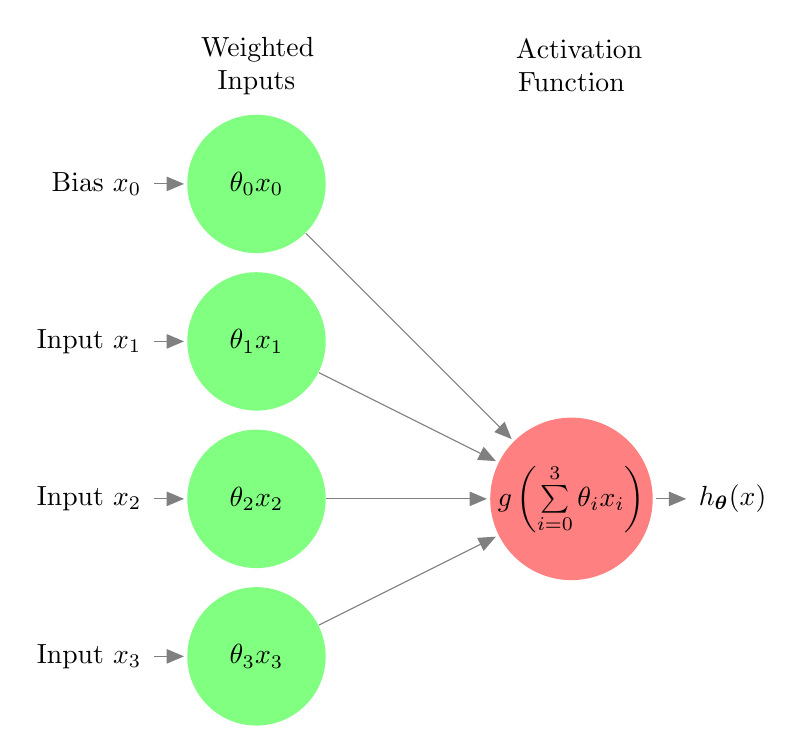
\begin{tikzpicture}[shorten >=1pt,->,draw=black!50, node distance=2.5cm]
    \tikzstyle{every pin edge}=[<-,shorten <=1pt]
    \tikzstyle{neuron}=[circle,fill=black!25,minimum size=50pt,inner sep=0pt]
    \tikzstyle{input neuron}=[neuron, fill=green!50];
    \tikzstyle{output neuron}=[neuron, fill=red!50];
    \tikzstyle{hidden neuron}=[neuron, fill=blue!50];
    \tikzstyle{annot} = [text width=4em, text centered]

    % Draw the input layer nodes
 %   \foreach \name / \y in {0,...,3}
    % This is the same as writing \foreach \name / \y in {1/1,2/2,3/3,4/4}
        \node[input neuron, pin=left:Bias $x_0$] (I-0) at (0,-0) {$\theta_0 x_0$};
	\foreach \name / \y in {1,...,3}
    % This is the same as writing \foreach \name / \y in {1/1,2/2,3/3,4/4}
        \node[input neuron, pin=left:Input $x_{\y}$] (I-\name) at (0,-2*\y) {$\theta_{\y}x_\y$};
    % Draw the hidden layer nodes
    %\foreach \name / \y in {1,...,5}
     %   \path[yshift=0.5cm]
      %      node[hidden neuron] (H-\name) at (\layersep,-\y cm) {};

    % Draw the output layer node
    \node[output neuron,pin={[pin edge={->}]right:$h_{\bm{\theta}}(x)$}, right of=I-2, node distance=4cm] (O) {$g\left(\sum\limits^3_{i=0}\theta_ix_i\right)$};

    % Connect every node in the input layer with every node in the
    % hidden layer.
   % \foreach \source in {1,...,4}
    %    \foreach \dest in {1,...,5}
     %       \path (I-\source) edge (H-\dest);

    % Connect every node in the hidden layer with the output layer
    \foreach \source in {0,...,3}
        \path (I-\source) edge (O);

    % Annotate the layers
%    \node[annot,above of=H-1, node distance=1cm] (hl) {Hidden layer};
    \node[annot,above of=I-0, node distance=1.5cm](il) {Weighted Inputs};
    \node[annot,right of=il, node distance=4cm] {Activation Function};
\end{tikzpicture}
\caption{Individual Node Structure}
\end{figure}
\newpage
Some common activation functions are\cite{DeepLearning}:
\begin{itemize}
\item The rectified linear unit or ReLU activation function output is bound in $[0,\infty)$. It has the formula $g(x)=\max\{0,x\}$ corresponding to node function $h_{\bm{\theta}}(\textbf{x})=\max\{0,\bm{\theta}^\top\textbf{x}\}$.
\item The sigmoid or logistic activation function outputs are restricted to $(0,1)$, with the formula $g(x)=(1+\exp(-x))^{-1}$ corresponding to node function  $h_{\bm{\theta}}(\textbf{x})=(1+\exp(-\bm{\theta}^\top\textbf{x}))^{-1}$.
\item The hyperbolic tangent function output ranges between $(-1,1)$, denoted as $g(x)=\tanh(x)$ corresponding to $h_{\bm{\theta}}(\textbf{x})=\tanh(\bm{\theta}^\top\textbf{x})$.
\item The linear activation function is used to describe nodes with no activation function, as its formula is $g(x)=x$, corresponding to $h_{\bm{\theta}}(\textbf{x})=\bm{\theta}^\top\textbf{x}$. It therefore ranges in $\R$.
\end{itemize}
Their plots are shown in Figure 2.2 below.\\
\begin{figure}[h]
\resizebox{\textwidth}{!}{
\begin{tikzpicture}
\begin{axis}[name=ReLU, xlabel=$x$, ylabel=$g(x)$, ymin=-0.5, ymax=2, xmin=-2, xmax=2, legend pos = north west]
\addplot [domain=-2:2, samples=100]{max(0,x)};
\addlegendentry{ReLU}
\end{axis}
\begin{axis}[name=Sigmoid, at=(ReLU.right of south east), anchor = left of south west, xlabel=$x$, ylabel=$g(x)$, ymin=-0.5, ymax=1.5, xmin=-2, xmax=2, legend pos = north west]
\addplot [domain=-2:2, samples=100]{1/(1+exp(-x))};
\addplot [dotted, domain=-2:2, samples=100]{1};
\addplot [dotted, domain=-2:2, samples=100]{0};
\addlegendentry{Sigmoid}
\end{axis}
\begin{axis}[name=Linear, at=(Sigmoid.below south west), anchor = above north west, xlabel=$x$, ylabel=$g(x)$, ymin=-2, ymax=2, xmin=-2, xmax=2, legend pos = north west]
\addplot [domain=-2:2, samples=100]{x};
\addlegendentry{Linear}
\end{axis}
\begin{axis}[name=Tanh, at=(Linear.left of south west), anchor = right of south east, xlabel=$x$, ylabel=$g(x)$, ymin=-1.5, ymax=1.5, xmin=-2, xmax=2, legend pos = north west]
\addplot [domain=-2:2, samples=100]{tanh(x)};
\addplot [dotted, domain=-2:2, samples=100]{1};
\addplot [dotted, domain=-2:2, samples=100]{-1};
\addlegendentry{Tanh}
\end{axis}
\end{tikzpicture}
}
\caption{Activation Function Plots}
\end{figure}
\newpage
The choice of activation function is mostly dependent on the desired range of the node's output. For example, if the node's output is the estimate of a probability (ranging in $(0,1)$), then the sigmoid function would be used. Before discussing this further, we first describe the overall neural network structure, as the choice of activation function is dependent on the node's relative location on the network.
\section{Neural Network Structure}
A typical neural network is made up of layers of interconnected nodes\cite{neuralstat}. The first layer, called the input layer, does not have an activation function or weights, rather it simply acts as an input interface for the network. The outputs from the nodes can only be sent to other nodes in succeeding layers, with the exception of the final output layer; its result is simply the output of the network. The layers of nodes between the input and output layer are the hidden layers, as their weights and outputs are not useful to the user. Hidden layers can have an arbitrary number of nodes, whilst the nodes in the input and output layers are restricted to the number of inputs and outputs the program has. Figure 2.3 below illustrates a simple neural network function $f_{\bm{\Theta}}(\bm{x})$ with 3 external inputs, 1 hidden layer with 3 nodes, 1 bias node per non-output layer and 1 output node. This example, along with the notations is described in Example 2.3.1 on the next page.
\begin{figure}[h]
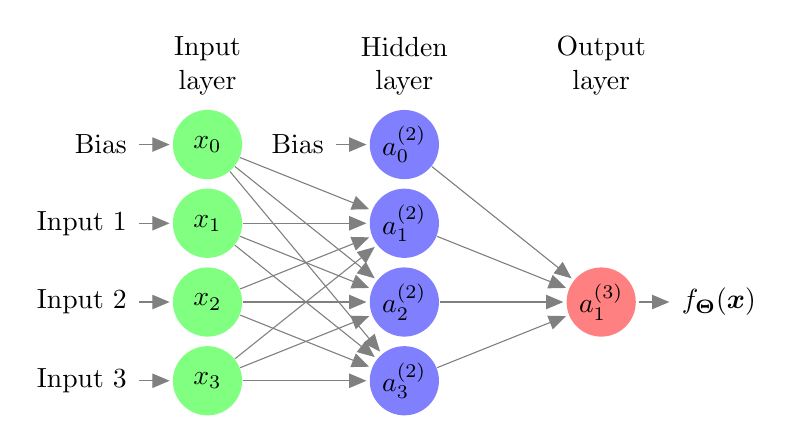
\begin{tikzpicture}[shorten >=1pt,->,draw=black!50, node distance=2.5cm]
    \tikzstyle{every pin edge}=[<-,shorten <=1pt]
    \tikzstyle{neuron}=[circle,fill=black!25,minimum size=25pt,inner sep=0pt]
    \tikzstyle{input neuron}=[neuron, fill=green!50];
    \tikzstyle{output neuron}=[neuron, fill=red!50];
    \tikzstyle{hidden neuron}=[neuron, fill=blue!50];
    \tikzstyle{annot} = [text width=4em, text centered]
    
	\node[input neuron, pin=left:Bias] (I-0) at (0,0) {$x_0$};
    % Draw the input layer nodes
    \foreach \name / \y in {1,...,3}
    % This is the same as writing \foreach \name / \y in {1/1,2/2,3/3,4/4}
        \node[input neuron, pin=left:Input \y] (I-\name) at (0,-\y) {$x_\y$};

 \path[yshift=0cm]
            node[hidden neuron, pin=left:Bias] (H-0) at (2.5cm,0) {$a^{(2)}_0$};
    % Draw the hidden layer nodes
    \foreach \name / \y in {1,...,3}
        \path[yshift=0cm]
            node[hidden neuron] (H-\name) at (2.5cm,-\y) {$a^{(2)}_\y$};

    % Draw the output layer node
	\path[yshift=1cm]    
    node[output neuron,pin={[pin edge={->}]right:$f_{\bm{\Theta}}(\bm{x})$}, right of=H-2] (O) {$a_1^{(3)}$};

    % Connect every node in the input layer with every node in the
    % hidden layer.
    \foreach \source in {0,...,3}
        \foreach \dest in {1,...,3}
            \path (I-\source) edge (H-\dest);

    % Connect every node in the hidden layer with the output layer
    \foreach \source in {0,...,3}
        \path (H-\source) edge (O);

    % Annotate the layers
    \node[annot,above of=H-0, node distance=1cm] (hl) {Hidden layer};
    \node[annot,left of=hl] {Input layer};
    \node[annot,right of=hl] {Output layer};
\end{tikzpicture}
\caption{Neural Network Structure}
\end{figure}
\newpage
\begin{example}
In this example, we denote the activation function as $g$, the output of node $i$ in layer $j$ as $a^{(j)}_i$, and the matrix of weights from layer $j$ to $j+1$ as $\Theta^{(j)}$. We also use the subscript $\Theta^{(j)}_{m,n}$ where $m$ is the row of the matrix corresponding to the node $m$ in layer $j+1$, and $n$ is the column of the matrix relating to node $n$ in layer $j$.\\
Individually, the outputs in the hidden nodes and the output node are:
\[x_0=1,\qquad a_0^{(2)}=1\]
\[a_1^{(2)}=g(\Theta^{(1)}_{1,0}x_0+\Theta^{(1)}_{1,1}x_1+\Theta^{(1)}_{1,2}x_2+\Theta^{(1)}_{1,3}x_3)\]
\[a_2^{(2)}=g(\Theta^{(1)}_{2,0}x_0+\Theta^{(1)}_{2,1}x_1+\Theta^{(1)}_{2,2}x_2+\Theta^{(1)}_{2,3}x_3)\]
\[a_3^{(2)}=g(\Theta^{(1)}_{3,0}x_0+\Theta^{(1)}_{3,1}x_1+\Theta^{(1)}_{3,2}x_2+\Theta^{(1)}_{3,3}x_3)\]
\[f_\Theta(\bm{x})=a_1^{(3)}=g(\Theta^{(2)}_{1,0}a_0^{(2)}+\Theta^{(2)}_{1,1}a_1^{(2)}+\Theta^{(2)}_{1,2}a_2^{(2)}+\Theta^{(2)}_{1,3}a_3^{(2)}).\]
Denoting the weights outputting to unit $i$ in layer $j+1$ as $\bm{\theta}^{(j)}_i = [\Theta_{i,0}^{(j)}\quad \Theta_{i,1}^{(j)}\cdots \Theta_{i,k}^{(j)}]^\intercal$ where $k+1$ is the number of inputs, we have the vectorized notation:
\[a_0^{(2)}=1\]
\[a_1^{(2)}=g((\bm{\theta}^{(1)}_1)^\intercal\bm{x})\]
\[a_2^{(2)}=g((\bm{\theta}^{(1)}_2)^\intercal\bm{x})\]
\[a_3^{(2)}=g((\bm{\theta}^{(1)}_3)^\intercal\bm{x})\]
\[f_{\bm{\theta}}(\bm{x})=a_1^{(3)}=g(\bm{\theta}^{(2)}_1)^\intercal\bm{a}^{(2)})\] 
where $\bm{a}^{(2)}=[a_0^{(2)}\quad a_1^{(2)}\quad a_2^{(2)}\quad a_3^{(3)}]^\intercal$.\\
An even simpler notation is:
\[a_0^{(2)}=1\]
\[[a_1^{(2)}\quad a_2^{(2)}\quad a_3^{(2)}]=g((\Theta^{(1)})^\intercal\bm{x})\]
\[f_{\bm{\Theta}} (\bm{x})=\bm{a}^{(3)}=g((\Theta^{(2)})^\intercal\bm{a}^{(2)}).\]
\end{example}
\newpage
\section{Bias-per-node Representation}
The use of a bias node leads to a minor programming inconvenience: the number of inputs in each layer is one more than the number of outputs of each node in the preceding layer. To make these values consistent, the bias node is often replaced with an intercept term added to the weighted input of a node before it passes through the activation function\cite{DeepLearning}. These intercept terms are optimized alongside the weights. In either case, the bias takes the form of a scalar added to the weighted inputs, which can be optimized. There is no practical difference between these two notations: the sum of intercept terms in a layer is equivalent to the weight corresponding to a bias node for the layer. Figures 2.4 and 2.5 below illustrate this concept, repeating the example of an individual node with three inputs, but with an individual intercept $b_i$ per node.\\
\begin{figure}[h]
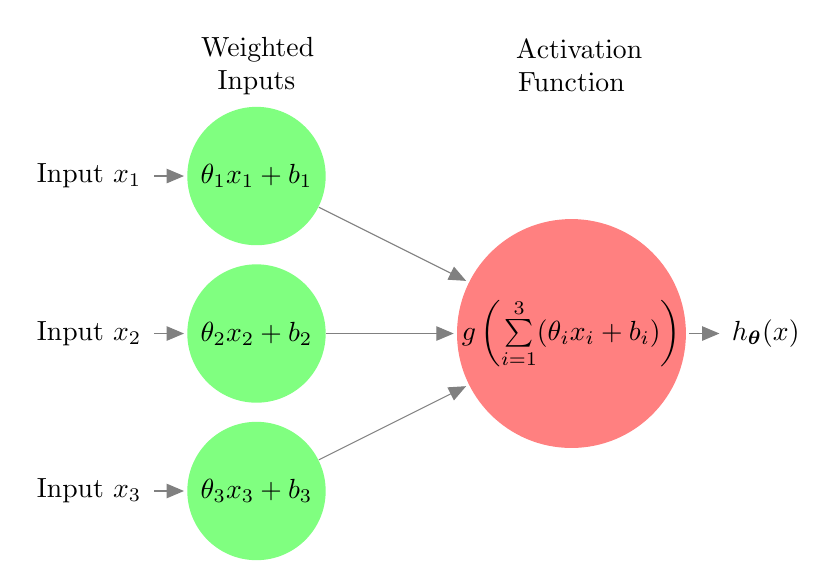
\begin{tikzpicture}[shorten >=1pt,->,draw=black!50, node distance=2.5cm]
    \tikzstyle{every pin edge}=[<-,shorten <=1pt]
    \tikzstyle{neuron}=[circle,fill=black!25,minimum size=50pt,inner sep=0pt]
    \tikzstyle{input neuron}=[neuron, fill=green!50];
    \tikzstyle{output neuron}=[neuron, fill=red!50];
    \tikzstyle{hidden neuron}=[neuron, fill=blue!50];
    \tikzstyle{annot} = [text width=4em, text centered]

    % Draw the input layer nodes
 %   \foreach \name / \y in {0,...,3}
    % This is the same as writing \foreach \name / \y in {1/1,2/2,3/3,4/4}
      %  \node[input neuron, pin=left:Bias $x_0$] (I-0) at (0,-0) {$\theta_0 x_0$};
	\foreach \name / \y in {1,...,3}
    % This is the same as writing \foreach \name / \y in {1/1,2/2,3/3,4/4}
        \node[input neuron, pin=left:Input $x_{\y}$] (I-\name) at (0,-2*\y) {$\theta_{\y}x_\y+b_\y$};
    % Draw the hidden layer nodes
    %\foreach \name / \y in {1,...,5}
     %   \path[yshift=0.5cm]
      %      node[hidden neuron] (H-\name) at (\layersep,-\y cm) {};

    % Draw the output layer node
    \node[output neuron,pin={[pin edge={->}]right:$h_{\bm{\theta}}(x)$}, right of=I-2, node distance=4cm] (O) {$g\left(\sum\limits^3_{i=1}(\theta_ix_i+b_i)\right)$};

    % Connect every node in the input layer with every node in the
    % hidden layer.
   % \foreach \source in {1,...,4}
    %    \foreach \dest in {1,...,5}
     %       \path (I-\source) edge (H-\dest);

    % Connect every node in the hidden layer with the output layer
    \foreach \source in {1,...,3}
        \path (I-\source) edge (O);

    % Annotate the layers
%    \node[annot,above of=H-1, node distance=1cm] (hl) {Hidden layer};
    \node[annot,above of=I-1, node distance=1.4cm](il) {Weighted Inputs};
    \node[annot,right of=il, node distance=4cm] {Activation Function};
\end{tikzpicture}
\caption{Individual Node Structure: Bias-per-node Representation}
\end{figure}
\begin{figure}[h]
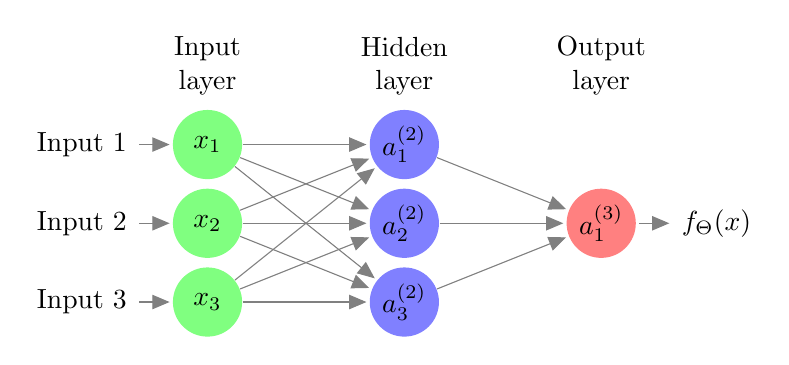
\begin{tikzpicture}[shorten >=1pt,->,draw=black!50, node distance=2.5cm]
    \tikzstyle{every pin edge}=[<-,shorten <=1pt]
    \tikzstyle{neuron}=[circle,fill=black!25,minimum size=25pt,inner sep=0pt]
    \tikzstyle{input neuron}=[neuron, fill=green!50];
    \tikzstyle{output neuron}=[neuron, fill=red!50];
    \tikzstyle{hidden neuron}=[neuron, fill=blue!50];
    \tikzstyle{annot} = [text width=4em, text centered]
    
	%\node[input neuron, pin=left:Bias] (I-0) at (0,0) {$x_0$};
    % Draw the input layer nodes
    \foreach \name / \y in {1,...,3}
    % This is the same as writing \foreach \name / \y in {1/1,2/2,3/3,4/4}
        \node[input neuron, pin=left:Input \y] (I-\name) at (0,-\y) {$x_\y$};

 %\path[yshift=0cm]
  %          node[hidden neuron, pin=left:Bias] (H-0) at (2.5cm,0) {$a^{(2)}_0$};
    % Draw the hidden layer nodes
    \foreach \name / \y in {1,...,3}
        \path[yshift=0cm]
            node[hidden neuron] (H-\name) at (2.5cm,-\y) {$a^{(2)}_\y$};

    % Draw the output layer node
	\path[yshift=1cm]    
    node[output neuron,pin={[pin edge={->}]right:$f_\Theta(x)$}, right of=H-2] (O) {$a_1^{(3)}$};

    % Connect every node in the input layer with every node in the
    % hidden layer.
    \foreach \source in {1,...,3}
        \foreach \dest in {1,...,3}
            \path (I-\source) edge (H-\dest);

    % Connect every node in the hidden layer with the output layer
    \foreach \source in {1,...,3}
        \path (H-\source) edge (O);

    % Annotate the layers
    \node[annot,above of=H-1, node distance=1cm] (hl) {Hidden layer};
    \node[annot,left of=hl] {Input layer};
    \node[annot,right of=hl] {Output layer};
\end{tikzpicture}
\caption{Neural Network Structure: Bias-per-node Representation}
\end{figure}
\newpage
Note here that $\sum^3_{i=1}b_i=\theta_0x_0$. The representation of the simple neural network example in Example 2.3.1 becomes:
\[a_1^{(2)}=g(\Theta^{(1)}_{1,1}x_1+b^{(1)}_1+\Theta^{(1)}_{1,2}x_2+b^{(1)}_2+\Theta^{(1)}_{1,3}x_3+b^{(1)}_3)\]
\[a_2^{(2)}=g(\Theta^{(1)}_{2,1}x_1+b^{(1)}_1+\Theta^{(1)}_{2,2}x_2+b^{(1)}_2+\Theta^{(1)}_{2,3}x_3+b^{(1)}_3)\]
\[a_3^{(2)}=g(\Theta^{(1)}_{3,1}x_1+b^{(1)}_1+\Theta^{(1)}_{3,2}x_2+b^{(1)}_2+\Theta^{(1)}_{3,3}x_3+b^{(1)}_3)\]
\[f_{\bm{\Theta}}(\bm{x})=a_1^{(3)}=g(\Theta^{(2)}_{1,1}a_1^{(2)}+b^{(2)}_1+\Theta^{(2)}_{1,2}a_2^{(2)}+b^{(2)}_2+\Theta^{(2)}_{1,3}a_3^{(2)}+b^{(2)}_3)\]
or in vectorized notation,
\[\bm{a}^{(2)}=g((\Theta^{(1)})^\intercal\bm{x})\]
\[f_{\bm{\Theta}}(\bm{x})=\bm{a}^{(3)}=g((\Theta^{(2)})^\intercal\bm{a}^{(2)})\]
\section{Choice of Activation Function}
In this section we describe the activation functions commonly used in the different layers of a neural network. Recall in section 2.2 the four most common activation functions are:
\begin{itemize}
\item The rectified linear unit or ReLU activation function $g(x)=\max\{0,x\}$ ranging in $[0,\infty)$.
\item The sigmoid or logistic activation function $g(x)=(1+\exp(-x))^{-1}$ restricted to $(0,1)$.
\item The hyperbolic tangent function $g(x)=\tanh(x)$ ranging between $(-1,1)$.
\item The linear activation function $g(x)=x$ ranging in $\R$.
\end{itemize}
Rectified linear units are the default choice for the hidden layers for their many advantages \cite{DeepLearning}
\begin{itemize}
\item Reduces overfitting: since negative ReLU inputs result in a zero output, on average only half of the units are "active" (non-zero output) when the network is first initialized. The proportion of active units can increase or decrease during training such that overfitting and underfitting is minimized.
\item Faster computation: a $\max\{0,x\}$ function is computed much faster than a function that uses $\exp$ or $\tanh$.
\item Easier and more consistent training: weight training in a neural network (discussed in Section 2.6) uses the gradient of overall node function, which is influenced by the activation function. The rectified linear unit has a consistent gradient $\theta$ or $0$ resulting in consistent training, as opposed to more complex units. Since the ReLU function is not differentiable at 0, the derivative $g'(0)$ is usually set to 0.
\end{itemize}
Since the input layer has no activation function, it can be described as having a linear activation function.\\
For the output layer, the activation function with the most reasonable output range is used. This depends on what the network is being used for. For example, in classification, the network assigns a probability to each case, so a sigmoid activation function would be most reasonable, as it ranges between 0 and 1. On the other hand, a rectified linear unit would be used for regression of a non-negative quantity such as price or time.
\section{Weight Initialization}
Proper initialization of the weights is ideal to improve convergence, as if the weights are too low, then the nodal outputs will continually decrease through the layers and become very small, requiring many iterations of training to fix. Similarly, if the weights are too high, then the result output of the network will be extremely large. In this section we discuss Xavier Initialization \cite{xavier}, which aims to keep the signal variance constant throughout the network. To derive the initialization algorithm, first consider in the bias-per-node representation a single node with $n$ inputs, and let $z$ denote the weighted sum of the inputs $\bm{\theta}^\top\textbf{x}$ before it is passed through the activation function. This is written as
\[z=\sum_{i=1}^n b_i+\sum^n_{i=1}\theta_ix_i.\]
$\sum_{i=1}^n b_i$ is a constant term, so $\Var(\sum_{i=1}^n b_i)=0$. Now under the assumption that the inputs and weights have 0 mean, we find the variance of the other terms:
\begin{align*}
Var(\theta_ix_i)&=\E[x_i]^2\Var(\theta_i)+\E[\theta_i]^2\Var(x_i)+\Var(\theta_i)\Var(x_i)\\
&=\Var(\theta_i)\Var(x_i).
\end{align*}
Assuming that the weights and inputs are also independent and identically distributed, we have
\[\Var(z)=n\Var(\theta_i)\Var(x_i).\]
Since we want constant variance of the signals throughout the network, we set $\Var(z)=\Var(x_i)$ and the result follows:
\[\Var(\theta_i)=\frac1n.\]
However, this result only considers forward propagation of the signal. A variation of this result accounts for back propagation by averaging the number of input and output nodes:
\[\Var(\theta_i)=\frac{2}{n_{in}+n_{out}}.\]
Thus, to enforce constant signal variance throughout the network, the ideal initialization of weights is to sample from a distribution, typically uniform or Gaussian, with $0$ mean and $\frac{2}{n_{in}+n_{out}}$ variance:
\[\theta_i\sim U\left(-\sqrt{\frac{6}{n_{in}+n_{out}}},\sqrt{\frac{6}{n_{in}+n_{out}}}\right)\]
or
\[\theta_i\sim N\left(0,\frac{2}{n_{in}+n_{out}}\right).\]
\section{Optimization}
The goal of optimizing the network is to train the weights of the network such that a loss function, which we will denote as $L$ as minimized. A common loss function is the squared error between the batch of network outputs and the actual results, so our objective function would be:
\[\min_\Theta L(\Theta)=\frac12 (\bm{y}-\bm{f}_\Theta(\bm{x}))^\top(\bm{y}-\bm{f}_\Theta(\bm{x})).\]
The $\frac12$ factor is included to eliminate the factor of 2 in the derivative, simplifying the derivations. The derivative is multiplied by an arbitrary training rate during optimization so there is no significant impact of including that term. \cite{DeepLearning}\\
The weights are initialized randomly, and through back-propagation (Section 2.8), their values are used to calculate the partial derivative of the loss function with respect to each individual weight (and bias). These partial derivatives are used in the gradient-based optimization of the weights. There are many variations of neural network optimization algorithms, but they are mostly based off gradient descent, which we will cover in this section.\cite{optimneural}\\
\begin{definition}
At point $\bm{x}^{(n)}$, $\bm{s}^{(n)}$ is a descent direction if $\nabla f\left(\bm{x}^{(n)}\right)^\intercal \bm{s}^{(n)}<0$.
\end{definition}
Gradient descent \cite{optim} is an algorithm used to find the minimizer $\bm{x}^*$ of a function $f$ by iterating on an arbitrary point $\bm{x}^{(n)}$, taking steps proportional to a descent direction $\bm{s}^{(n)}$:
\[\bm{x}^{(n+1)}=\bm{x}^{(n)}+\alpha \bm{s}^{(n)},\qquad \alpha>0.\]
A simple diagram illustrating this is shown in Figure 2.6 above.
\begin{figure}
\centering
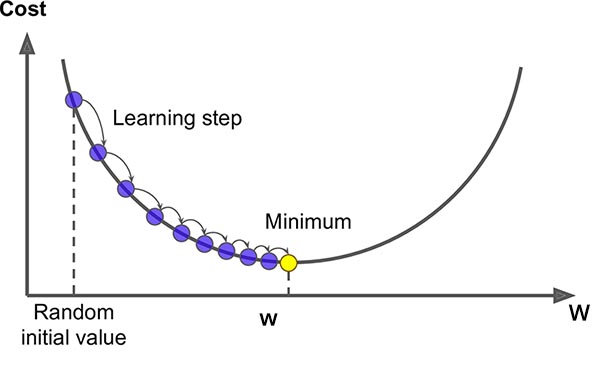
\includegraphics[scale=2]{gradientdescent.jpg}
\caption{Gradient Descent}
\end{figure}
\\
\begin{proposition} If $\bm{s}^{(n)}$ is a descent direction for $x^{(n)}$, then for small $\alpha>0$,
\[f(\bm{x}^{(n)}+\alpha \bm{s}^{(n)})<f(\bm{x}^{(n)}).\]
\begin{proof}
First we show that
\[\frac{d}{d\alpha}f(\bm{x}^{(n)}+\alpha \bm{s}^{(n)})=\nabla f(\bm{x}^{(n)}+\alpha \bm{s}^{(n)})^\intercal \bm{s}^{(n)}.\]
where $\bm{x}^{(n)}=[x_1^{(n)},\dots,x_k^{(n)}]^\top$ and $\bm{s}^{(k)}=[s_1^{(n)},\dots,s_k^{(n)}]^\top$.\\
Let
\[x_i^{(n)}(\alpha)=x_i^{(n)}+\alpha s_i^{(n)},\quad i=1,\dots,n\]
so that $\bm{x}^{(n)}+\alpha \bm{s}^{(n)}=[x_1^{(n)}(\alpha),\dots,x_k^{(n)}(\alpha)]^\intercal$.
We have
\begin{align*}
\frac{d}{d\alpha}f(\bm{x}^{(n)}+\alpha\bm{s}^{(n)})&= \frac{d}{d\alpha}f(x_1^{(n)},\dots,x_k^{(n)}(\alpha))\\
&= \sum^k_{i=1}\frac{\partial f(\bm{x})}{\partial x_i}|_{\bm{x}=\bm{x}^{(n)}+\alpha \bm{s}^{(n)}}\frac{d(x_i^{(n)}(\alpha))}{d\alpha}\\
&=\sum_{i=1}^k\frac{\partial f(\bm{x})}{\partial x_i}|_{\bm{x}=\bm{x}^{(n)}+\alpha \bm{s}^{(n)}}\bm{s}_i^{(n)}\\
%\frac{\partial f(\bm{x})}{\partial x_1}|_{\bm{x}=\bm{x}^{(n)}+\alpha \bm{s}^{(n)}}\bm{s}_1^{(n)}+\dots+\frac{\partial f(\bm{x})}{\partial x_n}|_{\bm{x}=\bm{x}^{(n)}+\alpha \bm{s}^{(n)}}\bm{s}_k^{(n)}\\
&=\nabla f(\bm{x}^{(n)}+\alpha \bm{s}^{(n)})^\intercal \bm{s}^{(n)}
\end{align*}
Setting $\alpha=0$ and using Definition 2.7.1,
\[\frac{d}{d\alpha}f(\bm{x}^{(n)}+\alpha\bm{s}^{(n)})|_{\alpha=0}=\nabla f(\bm{x}^{(n)})^\intercal \bm{s}^{(n)}<0\]
Therefore for small $\alpha>0$,
\[f(x^{(n)}+\alpha s^{(n)})<f(x^{(n)}).\]
\end{proof}
\end{proposition}
A common choice of descent direction is the negative of the gradient, that is, $-\nabla f(\bm{x}^{(n)})$, leading to the method of steepest descent. It is clearly a descent direction as $-\nabla f(\bm{x}^{(n)})^\intercal\nabla f(\bm{x}^{(n)})=-||\nabla f(\bm{x}^{(n)})||^2<0$.\\
By nature, gradient descent is guaranteed to converge to a local minimum, which is problematic if the function has local minima which differ from the global minima. This is not an issue in this thesis, as all the loss functions we use are convex, so any local minima are also global minima. Those interested in global optimization can refer to Deterministic Global Optimization by Floudas\cite{floudas}. When training a neural network on a non-convex loss function there are currently no commonly used methods of guaranteeing a global minimum, but the path may escape from a local minimum if randomness is introduced to the training process. This can be accomplished by stochastic gradient descent.\\
Typically, the entire batch of data is used in each iteration to calculate the loss function and gradient values required for gradient descent. This method of batch gradient descent is very slow for large datasets, and as previously described, its smoothness can cause the algorithm to converge to local minima. In stochastic gradient descent, only one observation is used per iteration, so the latent randomness associated with each observation effectively leads to noise added to each step, and the optimization is much faster. In practice, a compromise between stochastic and batch gradient descent is typically used; mini-batch gradient descent involves using several observations per iteration, leading to a reduction in the gradient variance\cite{optimneural}.\\
Gradient descent convergence can be improved by using an adaptive learning rate (ie. decreasing $\alpha$ over the iterations), as a low learning rate in the process will make convergence slow, whilst a high learning rate can cause the algorithm to oscillate around the minima\cite{optimneural}.\\
The Adam algorithm \cite{adam} incorporates these two concepts to form an effective optimization algorithm that is commonly applied to neural networks. In this thesis, we use this algorithm, but omit the specifics.
\section{Back-Propagation}
In the back-propagation algorithm, the goal is to find the partial derivative of the loss function with respect to the individual weights \[\frac{\partial}{\partial\Theta_{m,n}^{(j)}}L(\Theta),\]
so that gradient descent can be performed to optimize the weights.\cite{backprop} For each training sample $(\bm{x}^{(I)},\bm{y}^{(I)})$, $I=1,\dots,N$, the input signal is propagated forward throughout the network to calculate $\bm{a}^{(j)}$ for $j=2,\dots,J$, where $J$ is the total number of layers. The difference between the network output and the ideal result is calculated with 
\[\bm{\delta}^{(J)}=\bm{a}^{(J)}-\bm{y}^{(I)},\] 
and this error is propagated backwards through the network to find $\bm{\delta}^{(J-1)},\dots,\bm{\delta}^{(2)}$ by using the formula 
\[\bm{\delta}^{(j)}=((\Theta^{(j)})^\top \bm{\delta}^{(j+1)}).*g'(\Theta^{(j)^\top} \bm{a}^{(j)}),\] 
where $.*$ denotes element-wise multiplication and $g'$ is the derivative of the activation function. In this case, $g'$ takes in the sum of its weighted inputs, and as an example, the sigmoid activation function has the derivative $g'(\Theta^{(j)^\top} \bm{a}^{(j)})=\bm{a}^{(j)}.*(1-\bm{a}^{(j)})$. Note that $\bm{\delta}^{(1)}$ does not need to be calculated as the input layer is not weighted. \\
The errors for each layer are multiplied by each of the preceding layer's activation outputs to form the estimated partial derivative for the training sample. This result is added to an accumulator matrix, so that the average partial derivative from all the training samples can be computed:
\[\Delta^{(j)}_{m,n}:=\Delta^{(j)}_{m,n}+a_n^{(j)}\delta_m^{(j+1)}\]
or in matrix-vector form.
\[\Delta^{(j)}:=\Delta^{(j)}+\bm{\delta}^{(j+1)}(\bm{a}^{(j)})^\top.\]
Finally, we divide the accumulator matrix entries by the number of training samples to find the average partial derivative of the cost function with respect to the weights:
\[\frac{\partial}{\partial \Theta^{(j)}_{m,n}}L(\Theta)=\frac1N \Delta_{m,n}^{(j)}.\]
When $n\neq0$ (i.e. not considering the bias node), we can optionally add a regularizer term $\lambda > 0$ which decreases the magnitude of the weights, preventing overfitting \cite{DeepLearning}
\[\frac{\partial}{\partial \Theta^{(j)}_{m,n}}L(\Theta)=\frac1N (\Delta_{m,n}^{(j)}+\lambda \Theta_{m,n}^{(j)}).\]
There is no significant change when the bias node is regularized.\\
Pseudocode for back-propagation is shown in Algorithm 1 on the next page.\\
\begin{algorithm}
\caption{Back-Propagation Algorithm}
\KwData{Training Data $\{(\bm{x}^{(1)},\bm{y}^{(1)}),\dots ,(\bm{x}^{(N)},\bm{y}^{(N)})\}$, Regularizer Term $\lambda$}
\KwResult{Cost Function Partial Derivatives $\frac{\partial}{\partial\Theta^{(j)}_{m,n}}L(\Theta)$}
\BlankLine
\Begin{Randomly initialize weights $\Theta$\;
Set $\Delta^{(j)}_{m,n}=0 \quad \forall j,m,n$\;
\For{$I=1$ \KwTo $N$}{
Set $\bm{a}^{(1)}=\bm{x}^{(I)}$\;
\For{$j=2$ \KwTo $J$}{
Set $\bm{a}^{(j)}=\Theta^{(j-1)^\top}\bm{a}^{(j-1)}$\;}
Set $\bm{\delta}^{(J)}=\bm{a}^{(J)}-\bm{y}^{(I)}$\;
\For{$j=J-1$ \KwTo $2$}{
Set $\bm{\delta}^{(j)}=((\Theta^{(j)})^\top \bm{\delta}^{(j+1)}).*g'(\Theta^{(j)^\top}\bm{a}^{(j)})$\;
}
\For{$j=1$ \KwTo $J-1$}{
Set $\Delta^{(j)}=\Delta^{(j)}+\bm{\delta}^{(j+1)}(\bm{a}^{(j)})^\top$\;
}}
\For{all $j,m,n$}{
\eIf{$n=0$}{Set $\frac{\partial}{\partial\Theta^{(j)}_{m,n}}L(\Theta)=\frac1N \Delta^{(j)}_{m,n}$\;
}{Set $\frac{\partial}{\partial\Theta^{(j)}_{m,n}}L(\Theta)=\frac1N (\Delta^{(j)}_{m,n}+\lambda\Theta^{(j)}_{m,n})$\;}}}
\end{algorithm}
Having derived the partial derivatives of the loss function with respect to the individual weights, we can use a gradient descent based optimization method to update the weights. The partial derivatives are re-calculated after each optimization update until convergence is achieved.
\chapter{Variational Inference}
In this chapter, we explain variational inference, a method that uses a different, `variational' distribution to approximate posterior distributions in the context of Bayesian statistics. The name comes from the use of variational calculus to derive certain expressions. We first describe the Bayesian framework and problems associated with computational intractability. We then explain, with examples, two types of variational inference: mean-field variational inference and amortized inference. Finally, the chapter is concluded with a description of issues that arise when one or more of the prior or likelihood distributions are implicit, that is, their parametrisation is unknown but it is possible to sample from them.
\section{Context}
A fundamental problem in Bayesian statistics is to evaluate, or estimate posterior densities to perform analysis on unknown parameters \cite{gelman}. Consider the set of latent and known variables $z_1,\dots,z_M$ and $x_1,\dots,x_N$, respectively, with joint density $p(\textbf{z},\textbf{x})$. The posterior density $p(\textbf{z}|\textbf{x})$ is the distribution of the latent parameters $z_1,\dots,z_M$ conditioned on the known variables $\textbf{x}$. Applying Bayes' theorem, it can be written as:
\begin{equation*}
p(\textbf{z}|\textbf{x})=\frac{p(\textbf{z},\textbf{x})}{p(\textbf{x})}= \frac{p(\textbf{z})p(\textbf{x}|\textbf{z})}{\int_\mathbcal{z}p(\textbf{z},\textbf{x})d\textbf{z}}
\end{equation*}
where
\begin{itemize}
\item $p(\textbf{z})$ is the prior distribution: the initial distribution of $\textbf{z}$ before the data $\textbf{x}$ is observed. This can be initialised to represent our initial beliefs, or it can be parametrised randomly,
\item $p(\textbf{x}|\textbf{z})$ is the likelihood: the distribution of data $\textbf{x}$ conditioned on the parameters $\textbf{z}$,
\item $p(\textbf{x})=\int_\mathcal{z}p(\textbf{z},\textbf{x})d\textbf{z}$ is the marginal likelihood, or the evidence: the density of the data averaged across all possible parameter values.
\end{itemize}
If the evidence integral $p(\textbf{x})=\int_\mathbcal{z}p(\textbf{z},\textbf{x})d\textbf{z}$ is computationally intractable, then we are unable to evaluate the posterior density. Traditional MCMC (Markov Chain Monte Carlo) methods overcome this obstacle by sampling from a Markov chain that converges to the stationary distribution $p(\textbf{z},\textbf{x})$. However, these methods tend to have slow convergence for large datasets or complex models. When faced with these issues or when desiring a faster computation, one may instead apply variational inference, an alternative approach to density estimation. Variational inference methods can be much faster than MCMC, but they are known to underestimate the true posterior variance\cite{blei}, leading to a trade-off between speed of convergence and mean squared error.

\section{The KL Divergence}
We now present the KL (Kullback-Leibler) divergence, a type of f-divergence that is commonly used in variational inference. It is a measure of how much two probability distributions differ\cite{KL}.
\begin{definition}
The KL divergence is the expected logarithmic difference between two distributions $P$ and $Q$ with respect to $P$:
\begin{equation*}
KL(p(x)||q(x))=\int_{-\infty}^\infty p(x)\log \left(\frac{p(x)}{q(x)}\right)dx=\mathbb{E}_{p(x)}\left[\log\left(\frac{p(x)}{q(x)}\right)\right].
\end{equation*}
\end{definition}
\begin{remark}
The KL divergence is not symmetric:
\begin{equation*}
KL(p(x)||q(x))\neq KL(q(x)||p(x)).
\end{equation*}
\end{remark}
In variational inference, $KL(p(x)||q(x))$ is known as the forward KL divergence, whilst $KL(q(x)||p(x))$ is the reverse KL divergence. The expectation is taken with respect to different distributions.
\begin{lemma}
The KL divergence is non-negative, and it is equal to zero if and only if $p(x)=q(x)$ for almost all $x$:
\begin{equation*}
KL(q(x)||p(x))\geq 0.
\end{equation*}
We prove this in the case where $P$ and $Q$ are continuous distributions: a similar proof holds when they are discrete.
\begin{proof}
In the third line we use $\log x \leq x-1 \quad \forall x>0$ with equality if and only if $x=1$, therefore $KL(q(x)||p(x))=0$ if and only if $q(x)=p(x)$. The last line is due to $p(x)$ and $q(x)$ being probability densities.
\begin{align*}
KL(p(x)||q(x))&=\int_{-\infty}^\infty p(x)\log \left(\frac{p(x)}{q(x)}\right)dx\\
&=-\int_{-\infty}^\infty p(x)\log \left(\frac{q(x)}{p(x)}\right)dx\\
&\geq -\int_{-\infty}^\infty p(x) \left(\frac{q(x)}{p(x)}-1\right)dx\\
&=-\int_{-\infty}^\infty q(x)dx + \int_{-\infty}^\infty p(x)dx\\
&=0
\end{align*}
\end{proof}
\end{lemma}
\section{Introduction to Variational Inference}
Variational inference approximates the true posterior distribution $p(\textbf{z}|\textbf{x})$ with a different distribution $q(\textbf{z})$, taken from a tractable family of approximate distributions $\mathcal{Q}$, and then minimizes the f-divergence between the two distributions in an optimization problem:
\begin{equation}
q^*(\textbf{z})=\argmin_{q(\textbf{z})\in \mathcal{Q}}D_f(q(\textbf{z})||p(\textbf{z}|\textbf{x}))
\end{equation} where $D_f$ denotes an f-divergence\cite{blei}. This produces an analytic approximation to the posterior density. The most common f-divergence used in variational inference is the reverse KL divergence, used instead of the forward KL divergence as we are unable to sample from our true posterior $p(z|x)$, and because it leads to an expectation maximization algorithm as opposed to an expectation propagation algorithm. Equation 3.3.1 can therefore be written as:
\begin{equation}
q^*(\textbf{z})=\argmin_{q(\textbf{z})\in \mathcal{Q}}KL(q(\textbf{z})||p(\textbf{z}|\textbf{x})).
\end{equation}
From lemma 3.2.3, it is evident that $KL(q(\textbf{z})||p(\textbf{z}|\textbf{x}))$ attains a minimal value of $0$ when $q(\textbf{z})=p(\textbf{z}|\textbf{x})$.\\
There is an issue with solving equation 3.3.2 directly: we cannot evaluate the reverse KL divergence as $p(\textbf{z}|\textbf{x})$ is unknown, a result of $p(\textbf{x})$ being intractable. Instead, we rearrange the terms of equation 3.3.2 to formulate a tractable expression that can be optimized.

\section{Derivation of the ELBO}
In this section, we formulate the evidence lower bound (ELBO) of our posterior inference problem. Maximisation of this term is equivalent to solving equation 3.3.2. We begin by applying Bayes' law to the problem and expanding the terms:
\begin{align*}
q^*(\textbf{z})&=\argmin_{q(\textbf{z})\in \mathcal{Q}}KL(q(\textbf{z})||p(\textbf{z}|\textbf{x}))\\
&= \argmin_{q(\textbf{z})\in \mathcal{Q}} \mathbb{E}_{q(\textbf{z})}[\log q(\textbf{z})-\log p(\textbf{z}|\textbf{x})]\\
&= \argmin_{q(\textbf{z})\in \mathcal{Q}} \mathbb{E}_{q(\textbf{z})}\left[\log q(\textbf{z})-\log\frac{p(\textbf{x}|\textbf{z})p(\textbf{z})}{p(\textbf{x})}\right]\\
&= \argmin_{q(\textbf{z})\in \mathcal{Q}} \left(\mathbb{E}_{q(\textbf{z})}[\log q(\textbf{z})-\log p(\textbf{x}|\textbf{z})-\log p(\textbf{z})]+\log p(\textbf{x})\right).
\end{align*}
Note in the last line $\mathbb{E}_{q(\textbf{z})}[p(\textbf{x})]=p(\textbf{x})$ as it is not dependent on $q(\textbf{z})$. Since our issues with equation 3.3.2 result from the intractability of $p(\textbf{x})$, we rearrange the KL divergence expression as follows:
\begin{align}
KL(q(\textbf{z})||p(\textbf{z}|\textbf{x}))&=\mathbb{E}_{q(\textbf{z})}[\log q(\textbf{z})-\log p(\textbf{x}|\textbf{z})-\log p(\textbf{z})]+\log p(\textbf{x}) \nonumber \\
\log p(\textbf{x})-KL(q(\textbf{z})||p(\textbf{z}|\textbf{x}))&=-\mathbb{E}_{q(\textbf{z})}[\log q(\textbf{z})-\log p(\textbf{x}|\textbf{z})-\log p(\textbf{z})]\nonumber \\
&=\mathbb{E}_{q(\textbf{z})}[\log p(\textbf{x}|\textbf{z})]-\mathbb{E}_{q(\textbf{z})}[\log q(\textbf{z})-\log p(\textbf{z})]\nonumber \\
&=\mathbb{E}_{q(\textbf{z})}[\log p(\textbf{x}|\textbf{z})]-KL(q(\textbf{z})||p(\textbf{z})).
\end{align}
We refer to $\log p(\textbf{x})-KL(q(\textbf{z})||p(\textbf{z}|\textbf{x}))$ as $ELBO(q)$, as it is equal to the marginal probability of the data subtracted by a constant `error term'. Now our problem of minimizing the KL divergence between $q(\textbf{z})$ and $p(\textbf{z}|\textbf{x})$ is equivalent to maximizing $ELBO(q)$, which is equal to the tractable expression on line 3.4.1. We can therefore rewrite our optimization problem as:
\begin{align*}
q^*(\textbf{z})&=\argmin_{q(\textbf{z})\in \mathcal{Q}}KL(q(\textbf{z})||p(\textbf{z}|\textbf{x}))\\
&= \argmax_{q(\textbf{z})\in \mathcal{Q}} ELBO(q)\\
&= \argmax_{q(\textbf{z})\in \mathcal{Q}} \left(\mathbb{E}_{q(\textbf{z})}[\log p(\textbf{x}|\textbf{z})]-KL(q(\textbf{z})||p(\textbf{z}))\right).
\end{align*}
Note that this expression attains a maximum at the marginal likelihood of the dataset $\log p(\textbf{x})$, hence we may use the ELBO to construct a model selection criterion.
\newpage
\section{Mean-Field Variational Family}
The family of variational distributions $\mathcal{Q}$ is typically a `mean-field variational family', in which the distribution $q(\textbf{z})$ factorizes over the latent variables $\{z_i\}^M_{i=1}$, each with an individual set of parameters $\{\phi_i\}^M_{i=1}$:
\begin{equation}
q(\textbf{z})=\prod^M_{i=1}q_{\phi_i}(z_i).
\end{equation}
The individual factors $q_{\phi_i}(z_i)$ can take any form, but they are assumed to be independent, which simplifies derivations but is less accurate when the true latent variables exhibit dependence. Fixing the forms of the individual factors, we want to choose the parameters $\phi_i$ so that $ELBO(q)$ is maximized. To derive an expression for the optimal factor $q_i^*(z_i)$, we substitute equation 3.5.1 into the $ELBO$, factor out a specific $q_j(z_j)$ and equate the functional derivative of the resulting Lagrangian equation with 0. \\
Firstly, we express $ELBO(q)$ in an integral form as follows:
\begin{align*}
ELBO(q)&= \mathbb{E}_{q(z)}[\log p(\textbf{x}|\textbf{z})]-KL(q(\textbf{z})||p(\textbf{z}))\\
&= \mathbb{E}_{q(x)}[\log p(\textbf{x}|\textbf{z})+\log p(\textbf{z})-\log q(\textbf{z})]\\
&= \mathbb{E}_{q(z)}[\log p(\textbf{x}, \textbf{z})-\log q(\textbf{z})]\\
&= \int_{\mathbcal{z}}q(\textbf{z})(\log p(\textbf{x},\textbf{z})-\log q(\textbf{z}))d\textbf{z}.
\end{align*}
Substituting $q(\textbf{z})=\prod^M_{i=1}q_i(z_i)$ and factoring out $q_j(z_j)$ yields:
\begin{align}
ELBO(q)&= \int_\mathbcal{z}\left[\prod^M_{i=1}q_i(z_i)\right]\left(\log p(\textbf{x},\textbf{z})-\sum_{i=1}^M\log q_i(z_i)\right)d\textbf{z}\nonumber\\
&= \int_\mathcal{z_j}q_j(z_j)\left(\int_\mathcal{z_{-j}}\log p(\textbf{x},\textbf{z})\prod_{i\neq j}q_i(z_i)d\textbf{z}_{-j} \right) dz_j\nonumber\\
&\quad -\int_{\mathcal{z_j}}q_j(z_j)\left(\int_{\mathcal{z}_{-j}}\left[\prod_{i\neq j}q_i(z_i)\right]\sum_{i=1}^M q_i(z_i)d\textbf{z}_{-j}\right)dz_j\nonumber\\
&= \int_{\mathcal{z_j}}q_j(z_j)\mathbb{E}_{\textbf{z}_{-j}}[\log p(\textbf{x},\textbf{z})]dz_j\nonumber\\
&\quad -\int_{\mathcal{z_j}}q_j(z_j)\log q_j(z_j)\left(\int_{\mathcal{z}_{-j}}\prod_{i\neq j}q_i(z_i)dz_{-j}\right) dz_j\nonumber\\
&\quad -\int_{\mathcal{z_j}}q_j(z_j)\left(\int_{\mathcal{z}_{-j}}\left[\prod_{i\neq j}q_i(z_i)\right]\sum_{i\neq j}q_i(z_i)d{\textbf{z}_{-j}}\right)dz_j\nonumber\\
&= \int_\mathcal{z_j}q_j(z_j)\mathbb{E}_{\textbf{z}_{-j}}[\log p(\textbf{x},\textbf{z})]dz_j-\int_\mathcal{z_j}q_j(z_j)\log q_j(z_j)dz_j\nonumber\\
&\quad -\int_{\mathcal{z}_{-j}}\left[\prod_{i\neq j}q_i(z_i)\right]\sum_{i\neq j}q_i(z_i)d{\textbf{z}_{-j}}
\\&= \int_\mathcal{z_j}q_j(z_j)\left(\mathbb{E}_{\mathcal{z}_{-j}}[\log p(\textbf{x},\textbf{z})]-\log q_j(z_j)\right)dz_j+\text{const}.
\end{align}
The term in line 3.5.2 is a constant with respect to $q_j(z_j)$. We want to maximize $ELBO(q)$, so we formulate the Lagrangian equation with the constraint that $q_i(z_i)$ are probability density functions:
\begin{equation*}
ELBO(q)-\sum^M_{i=1}\lambda_i\int_\mathcal{z_i}q_i(z_i)dz_i=0
\end{equation*}
or using our expression for $ELBO(q)$ in line 3.5.3,
\begin{equation}
\int_\mathcal{z_j}q_j(z_j)\left(\mathbb{E}_{\mathcal{z}_{-j}}[\log p(\textbf{x},\textbf{z})]-\log q_j(z_j)\right)dz_j-\sum^M_{i=1}\lambda_i\int_\mathcal{z_i}q_i(z_i)dz_i+\text{const}=0.
\end{equation} 
We then take the functional derivative of Equation 3.5.4 with respect to $q_j(z_j)$:
\begin{align}
\frac{\partial ELBO(q)}{\partial q_j(z_j)}&= \frac{\partial}{\partial q_j(z_j)}\left[q_j(z_j)\left(\mathbb{E}_{\textbf{z}_{-j}}[\log p(\textbf{x},\textbf{z})]-\log q_j(z_j)\right)-\lambda_jq_j(z_j)\right]\nonumber
\\&= \mathbb{E}_{\textbf{z}_{-j}}[\log p(\textbf{x},\textbf{z})]-\log q_j(z_j)-1-\lambda_j.
\end{align}
Equating expression 3.5.5 to 0 and observing that $1+\lambda_j$ is constant with respect to $z$, we have:
\begin{align}
\log q_j^*(z_j)&= \mathbb{E}_{\textbf{z}_{-j}}[\log p(\textbf{x},\textbf{z})]-\text{const} \nonumber\\
q_j^*(z_j)&=\frac{e^{\mathbb{E}_{\textbf{z}_{-j}}[\log p(\textbf{x},\textbf{z})]}}{\exp{(\text{const})}}\nonumber\\
&= \frac{e^{\mathbb{E}_{\textbf{z}_{-j}}[\log p(\textbf{x},\textbf{z})]}}{\int e^{\mathbb{E}_{\textbf{z}_{-j}}[\log p(\textbf{x},\textbf{z})]}dz_j}.
\end{align}
\newpage
The normalization constant on the denominator of 3.5.6 is derived by observing $q^*_j(z_j)$ as a density. Finally, we derive a simpler expression of $q^*_j(z_j)$ by observing that terms independent of $z_j$ can be treated as a constant:
\begin{align}
q^*_j(z_j)&\propto \exp\left(\mathbb{E}_{\textbf{z}_{-j}}[\log p(\textbf{x},\textbf{z})]\right)\nonumber\\
&\propto \exp\left(\mathbb{E}_{\textbf{z}_{-j}}[\log p(z_j|\textbf{z}_{-j},\textbf{x})]\right).
\end{align}
This expression can be used in an expectation-maximization algorithm, in which the $q^*_j(z_j)$ is evaluated and iterated from $j=1\dots M$. This particular algorithm is called coordinate ascent variational inference (CAVI) (Algorithm 2):\\
\\
\begin{algorithm}[H]
\caption{Coordinate Ascent Variational Inference (CAVI)}
\KwData{Dataset $\textbf{x}$ and Bayesian Model p($\textbf{x},\textbf{z}$)}
\KwResult{Variational density $q(\textbf{z})=\prod^M_{i=1}q_i(z_i)$}
\BlankLine
\Begin{
Initialize random variational factors $q_j(z_j)$\;
\While{ELBO(q) has not converged}{

	\For{$j=1$ \KwTo $m$}{
	Set $q_j(z_j)\propto \exp(\mathbb{E}_{\textbf{z}_{-j}}[\log p(z_j|\textbf{z}_{-j},\textbf{x})])$\;
	}
	Calculate $ELBO(q)=\mathbb{E}_{q(\textbf{z})}[\log p(\textbf{z},\textbf{x})]-\mathbb{E}_{q(\textbf{z})}[\log q(\textbf{z})]$\;
}
Return $q(\textbf{z})$\;
}
\end{algorithm}
\newpage
\section{Example: Bayesian Mixture of Gaussians}
To illustrate the mean-field variational inference approach, we closely follow the Bayesian mixture of Gaussians example from Variational Inference: A Review for Statisticians by Blei \cite{blei}.\\
Consider the hierarchical model
\begin{align*}
\mu_k&\sim N(0,\sigma^2), &&k=1,\dots,K,\\
c_i&\sim \text{Categorical}\left(\frac{1}{K},\dots,\frac{1}{K}\right), &&i=1,\dots,n,\\
x_i|c_i,\bm{\mu}&\sim N(c^\top_i\bm{\mu},1), &&i=1,\dots,n.
\end{align*}
This is a Bayesian mixture of univariate Gaussian random variables with unit variance. In this model, we draw $K$ $\mu_k$ variables from a prior Gaussian distribution $N(0,\sigma^2)$ ($\sigma^2$ is a hyperparameter), forming the vector $\bm{\mu}=(\mu_1,\dots,\mu_K)^\top$. We then generate an indicator vector $c_i$ of length $K$ from a prior categorical distribution. This vector has zeros for every element except for one element, where it is a $1$. Each element has equal probability $1/K$ of being the element that contains the $1$. The transpose of this $c_i$ is then multiplied by $\bm{\mu}$, essentially choosing one of the $\bm{\mu}$ elements at random. We then draw $x_i$ from the resulting $N(c^\top_i\bm{\mu},1)$.\\
Here, our latent variables are $\textbf{z}=\{\textbf{c},\bm{\mu}\}$. Assuming $n$ samples, our joint density is
\begin{equation}
p(\bm{\mu},\textbf{c},\textbf{x})=p(\bm{\mu})\prod^n_{i=1}p(c_i)p(x_i|c_i, \bm{\mu}).\end{equation}
From this, we derive the marginal likelihood
\[p(\textbf{x})=\int p(\bm{\mu})\prod^n_{i=1}\sum_{c_i}p(c_i)p(x_i|c_i,\bm{\mu})d\bm{\mu}.\]
This integral is intractable, as the time complexity of evaluating it is $\mathcal{O}(K^n)$, which is exponential in $K$. To evaluate the posterior distribution over the latent variables $p(\bm{\mu},\textbf{c}|\textbf{x})$, we would have to apply variational inference, approximating it with a variational distribution $q(\bm{\mu},\textbf{c})$. We will assume this distribution follows the mean-field variational family:
\[q(\bm{\mu},\textbf{c})=\prod^K_{k=1}q(\mu_k;m_k,s^2_k)\prod^n_{i=1}q(c_i;\bm{\phi_i}).\]
In this distribution, we have $K$ Gaussian factors with mean $\mu_k$ and variance $s^2_k$, and $n$ categorical factors with index probabilities defined by the vector $\bm{\phi_i}$, such that
\begin{align*}
\mu_k&\sim N(m_k,s^2_k), &&k=1,\dots,K,\\
x_i&\sim \text{Categorical}(\bm{\phi_i}), &&i=1,\dots,n.
\end{align*}
Using this and equation 3.6.1, we can derive the evidence lower bound as a function of the variational parameters:
\begin{align*}
ELBO(\textbf{m},\textbf{s}^2,\bm{\phi})&=\mathbb{E}[\log p(\textbf{z},\textbf{x})]-\mathbb{E}[\log q(\textbf{z})]\\
&=\mathbb{E}[\log p(\bm{\mu,c},\textbf{x})]-\mathbb{E}[\log q(\bm{\mu,c})]\\
&=\sum^K_{i=1}\mathbb{E}[\log p(\mu_k); m_k,s^2_k]\\
&\quad +\sum^n_{i=1}\left(\mathbb{E}[\log p(c_i);\bm{\phi}_i]+\mathbb{E}[\log p(x_i|c_i,\bm{\mu});\bm{\phi}_i,\textbf{m},\textbf{s}^2]\right)\\
&\quad -\sum^K_{k=1}\mathbb{E}[\log q(\mu_k;m_k,s^2_k)]-\sum^n_{i=1}\mathbb{E}[\log q(c_i;\bm{\phi}_i)].
\end{align*}
From equation 3.5.7, we derive the optimal categorical factor by only considering terms from the true distribution $p(.)$ dependent on $c_i$:
\begin{equation}
q^*(c_i;\bm{\phi}_i)\propto \exp\left(\log p(c_i)+\mathbb{E}[\log p(x_i|c_i,\bm{\mu});\textbf{m},\textbf{s}^2]\right).
\end{equation}
Now since $c_i$ is an indicator vector,
\[p(x_i|c_i,\bm{\mu})=\prod^K_{k=1}p(x_i|\mu_k)^{c_{ik}}.\]
We can now evaluate the second term of equation 3.6.2:
\begin{align*}
\mathbb{E}\left([\log p(x_i|c_i,\bm{\mu});\textbf{m},\textbf{s}^2]\right)&=\sum_{k=1}^K c_{ik}\mathbb{E}[\log p(x_i|\mu_k);m_k,s^2_k]\\
&=\sum_{k=1}^K c_{ik}\mathbb{E}[-(x_i-\mu_k)^2/2;m_k,s^2_k]+\text{const}\\
&=\sum_{k=1}^Kc_{ik}\left(\mathbb{E}[\mu_k;m_k,s^2_k]x_i-\mathbb{E}[\mu^2_k;m_k,s^2_k]/2\right)+\text{const}.
\end{align*}
In each line, terms constant with respect to $c_{ik}$ have been taken out of the expression. Our optimal categorical factor becomes
\[q^*(c_i;\bm{\phi}_i)\propto \exp \left(\log p(c_i)+\sum_{k=1}^Kc_{ik}\left(\mathbb{E}[\mu_k;m_k,s^2_k]x_i-\mathbb{E}[\mu^2_k;m_k,s^2_k]/2\right)\right).\]
By proportionality, we then have the variational update
\[\phi_{ik}\propto \exp\left(\mathbb{E}[\mu_k;m_k,s^2_k]x_i-\mathbb{E}[\mu^2_k;m_k,s^2_k]/2\right).\]
Now we find the variational density of the $k$th mixture component, again using equation 3.5.7 with the ELBO and ignoring terms independent of $p(.)$ and $\mu_k$:
\[q(\mu_k;m_k,s^2_k)\propto \exp \left(\log p(\mu_k)+\sum^n_{i=1}\mathbb{E}[\log p(x_i|c_i,\bm{\mu});\phi_i, \textbf{m}_{-k},\textbf{s}^2_{-k}]\right).\]
The log of this density is
\begin{align*}
\log q(\mu_k)&=\log p(\mu_k)+\sum_i^n \mathbb{E}[\log p(x_i|c_i,\bm{\mu});\phi_i,\textbf{m}_{-k},\textbf{s}^2_{-k}]+\text{const}\\
&= \log p(\mu_k)+\sum_{i=1}^n\mathbb{E}[c_{ik}\log p(x_i|\mu_k);\phi_i]+\text{const}\\
&= -\frac{\mu^2_k}{2\sigma^2}+\sum^n_{i=1}\mathbb{E}[c_{ik};\phi_i]\log p(x_i|\mu_k)+\text{const}\\
&= -\frac{\mu^2_k}{2\sigma^2}+\sum^n_{i=1}\phi_{ik}\frac{-(x_i-\mu_k)^2}{2}+\text{const}\\
&= -\frac{\mu^2_k}{2\sigma^2}+\sum^n_{i=1} \phi_{ik}x_i\mu_k-\frac{\phi_{ik}\mu^2_k}{2}+\text{const}\\
&= \mu_k\left(\sum^n_{i=1}\phi_{ik}x_i\right)-\mu_k^2\left(\frac{1}{2\sigma^2}+\frac{\sum^n_{i=1}\phi_{ik}}{2}\right)+\text{const}\\
&= -\frac{1}{2}\left(\frac{1}{\sigma^2}+\sum^n_{i=1}\phi_{ik}\right)\left(\mu_k^2-\frac{2\sum^n_{i=1}\phi_{ik}x_i}{1/\sigma^2+\sum^n_{i=1}\phi_{ik}}\mu_k\right)+\text{const}
\end{align*}
The density is therefore
\[q(\mu_k)\propto \sqrt{\frac{1/\sigma^2+\sum^n_{i=1}\phi_{ik}}{2\pi}}\exp\left(-\frac{1}{2}\left(\frac{1}{\sigma^2}+\sum^n_{i=1}\phi_{ik}\right) \left(\mu_k-\frac{\sum^n_{i=1}\phi_{ik}x_i}{1/\sigma^2+\sum^n_{i=1}\phi_{ik}}\right)^2\right)\]
It can be seen that $q(\mu_k)$ is a Gaussian distribution, so our variational updates for $m_k$ and $s^2_k$ are its mean and variance:
\[m_k=\frac{\sum^n_{i=1}\phi_{ik}x_i}{1/\sigma^2+\sum^n_{i=1}\phi_{ik}}, \qquad s^2_k=\frac{1}{1/\sigma^2+\sum^n_{i=1}\phi_{ik}}.\]
We can now formulate the CAVI algorithm (Algorithm 3), which simply iterates the cluster assignment probabilities $\phi_{ik}$ and the variational density parameters $m_k$ and $s^2_k$ until the ELBO converges.
\begin{algorithm}
\caption{CAVI Algorithm for Bayesian mixture of Gaussians}
\KwData{Data $\textbf{x}$, Number of Gaussian components $K$, Hyperparameter value $\sigma^2$}
\KwResult{Optimal variational factors $q(\mu_k;m_k,s^2_k)$ and $q(c_i;\bm{\phi_i)}$}
\BlankLine
\Begin{
Randomly initialize parameters $\textbf{m}, \textbf{s}^2$ and $\bm{\phi}$\;
\While{ELBO has not converged}{
	\For{$i=1$ \KwTo $n$}{
		Set $\phi_{ik}\propto\exp\left(\mathbb{E}[\mu_k;m_k,s^2_k]x_i-\mathbb{E}			[\mu^2_k;m_k,s^2_k]/2\right)$\;
	}
	\For{$k=1$ \KwTo $K$}{
		Set $m_k=\frac{\sum_i\phi_{ik}x_i}{1/ \sigma^2+\sum_i\phi_{ik}}$\;
		Set $s^2_k=\frac{1}{1/ \sigma^2+\sum_i \phi_{ik}}$\;
	}
	Compute $ELBO(\textbf{m},\textbf{s}^2,\bm{\phi})$\;
}
Return $q(\textbf{m},\textbf{s}^2,\bm{\phi})$\;
}
\end{algorithm}
\newpage
\section{Amortized Inference}
One disadvantage of mean field variational inference is that a specific set of variational parameters needs to be derived and optimized for each data point. This can be computationally expensive for large datasets. Amortized inference resolves this issue by using a single, constant set of parameters for all data points, adding the data point itself as an input to the variational distribution \cite{ADVVI}. Our variational distribution therefore conditions on the observation, taking the form
\[q_\phi(z|x).\]
Figures 3.1 and 3.2 highlight the difference between mean-field and amortized variational inference. In the figures there are $N$ data points, and for each data point, $\bm{z}^{(i)}$ is $M$-dimensional. Therefore for mean-field variational inference, there are $M\times N$ sets of $\phi$ parameters, whilst in amortized inference there is only one set of $\phi$ parameters, as we use $M\times N$ data points as inputs.
\begin{figure}[h]
  \centering
  \tikz{ %
    \node[latent] (phi) {$\bm{\phi}^{(i)}$} ; %
    \node[latent, right=of phi] (z) {$\bm{z}^{(i)}$} ; %
    \plate[inner sep=0.25cm, xshift=-0.12cm, yshift=0.12cm] {plate1} {(phi) (z)} {$i\in 1:N$}; %
    \edge {phi} {z} ; %
   
  }
   \caption{DAG for Mean-Field Variational Inference}
\end{figure}
\begin{figure}[h]
\centering
  \tikz{ %
    \node[obs] (x) {$\bm{x}^{(i)}$} ; %
    \node[latent, above=of x] (phi) {$\bm{\phi}$} ; %
    \node[latent, right=of x] (z) {$\bm{z}^{(i)}$} ; %
    \plate[inner sep=0.25cm, xshift=-0.12cm, yshift=0.12cm] {plate1} {(x) (z)} {$i\in 1:N$}; %
    \edge {phi} {z} ; %
    \edge {x} {z} ;
    
  }
  \caption{DAG for Amortized Inference}
\end{figure}\\
Clearly, a very complex variational distribution is required to model such a structure, so it often takes the form of a neural network with $x$ as an input. This method is often used in deep learning due to the significant amount of data required to train such a network.\\

Now recall that $p(x)$ represents the marginal likelihood, or `true' distribution of the data. This is typically never available, we often instead have a sample dataset representing it. Denoting the dataset as $q^*(x)$, we want to optimize $\phi$ across the observations from our dataset, so our objective now is to choose parameters $\phi$ such that the expected KL divergence with respect to $q^*(x)$ is minimized:
\begin{align*}
\phi &=\argmin_\phi \mathbb{E}_{q^*(x)}KL(q_\phi(z|x)||p_\theta (z|x))\\
&= \argmin_\phi \mathbb{E}_{q^*(x)q_\phi (z|x)}\left[\log q_\phi(z|x)-\log p_\theta(z|x)\right]\\
&=\argmin_\phi\mathbb{E}_{q^*(x)q_\phi (z|x)}\left[\log q_\phi(z|x)-\log \frac{p(x|z)p(z)}{p(x)}\right]\\
&=\argmin_\phi\left(\mathbb{E}_{q^*(x)q_\phi (z|x)}\left[\log q_\phi(z|x)-\log p(x|z)-\log p(z)\right]+\log p(x)\right)
\end{align*} 
Again, we cannot evaluate this expression as $\log p(x)$ is intractable, so we rearrange the terms to form the evidence lower bound, which we want to maximise to minimise the KL divergence.
\begin{align*}
ELBO(q)&=\mathbb{E}_{q^*(x)}[\log p(x)-KL(q_\phi(z|x)||p_\theta(z|x))]\\
&=-\mathbb{E}_{q^*(x)q_\phi(z|x)}\left[\log q_\phi(z|x)-\log p(x|z)-\log p(z)\right]\\
&=\mathbb{E}_{q^*(x)q_\phi(z|x)}\left[\log p(x|z)+\log p(z)-\log q_\phi(z|x)\right]\\
&=\mathbb{E}_{q^*(x)}\left[\E_{q_\phi(z|x)}[\log p(x|z)]-KL(q_\phi(z|x)||p(z))\right]
\end{align*}
We take the negative to form the minimization problem of the negative evidence lower bound $NELBO(q)$:
\begin{equation}
\min_\phi NELBO(q)=\mathbb{E}_{q^*(x)}\left[-\E_{q_\phi(z|x)}[\log p(x|z)]+KL(q_\phi(z|x)||p(z))\right].
\end{equation}
Since $\phi$ represents the parameters of a neural network, it is inefficient to find the specific weight values during back-propagation: we are more interested in training the network to optimality, which occurs when we minimize the objective function. Hence, it is more appropriate to write the optimization problem with $\min$ than with $\argmin$.\\

In deep learning, the likelihood term is often represented as a neural network parametrized by $\theta$: $p_\theta(x|z)$. This network is optimized alongside the variational distribution, in a formation known as the variational autoencoder.
\newpage
\section{Example: Variational Autoencoder}
A variational autoencoder (Figure 3.3) is a model consisting of two simultaneously trained neural networks: an encoder $q_\phi(z|x)$ that ``compresses" a data point $x$ into a lower dimensional latent representation $z$, and a decoder $p_\theta(x|z)$ that ``reconstructs" the data point from the latent variable\cite{kingma}. It has two main purposes: representation learning of data and data generation. Typically, the prior $p(z)$ is simply a standard k-dimensional multivariate normal distribution $\mathcal{N}(0,I_{k\times k})$. We now reiterate our optimization problem in line 3.7.1, this time including the optimization of the decoder parameters $\theta$:
\[\min_{\phi,\theta} \mathbb{E}_{q^*(x)}\left[-\E_{q_\phi(z|x)}[\log p_\theta(x|z)]+KL(q_\phi(z|x)||p(z))\right].\]
The first term is the negative likelihood, which is analogous to the reconstruction error which we want to minimize. The KL divergence between the variational posterior and the true prior distribution acts as a regularizer term, encouraging the output of the posterior to be similar to a standard normal distribution. Without it, the encoder would learn to segregate distinct data types in separate regions of the Euclidean plane, which runs contrary to the properties of a probability distribution. We can therefore generate new data $x$ by sampling $z\sim p(z)$ and feeding it through the decoder.\\

At our current formulation, we have the problem that a neural network is deterministic, so for any given data point $x$, the encoder will always output the same $z$, which also contradicts the properties of a distribution. The solution is to have the encoder output a mean vector $\bm{\mu}=(\mu_1,\mu_2,\cdots,\mu_k)^\intercal$ and variance vector $\bm{\sigma}^2=(\sigma^2_1,\sigma^2_2,\cdots, \sigma^2_k)^\intercal$, each with dimensions equal to that of latent variable $z$. We have now defined $z$ as an output from a multivariate normal distribution with means and variances as specified by the encoder output:
\[q_\phi(z|x)\sim \mathcal{N}(\bm{\mu},\bm{\sigma}^2I_{k\times k}).\]
In practice, to reduce computational time, this is achieved by sampling random standard normal noise $\epsilon$, multiplying it by the variance and adding the result to the mean:
\[\epsilon\sim \mathcal{N}(0,I_{k\times k}),\qquad z=\mu+\epsilon\cdot\sigma^2.\]
\newpage
The expression in our optimization problem is tractable. It is often possible to parametrise an explicit form of the likelihood from the neural network output. For example, if $q^*(x)$ is a data set of grey-scale images, then a Bernoulli distribution can be used to represent the pixel values, with parameters given by the sigmoid output of the likelihood network. Since we have the explicit form of the multivariate normal $q_\phi(z|x)$ and $p(z)$ densities, the KL divergence term can be calculated through the equation:
\[KL(q(z|x)||p(z))=\frac12 \sum_{i=1}^k\left(\sigma^2_i+\mu^2_i-\log(\sigma^2_i)-1\right).\]
\begin{figure}[h]
  \centering
  \tikz{ %
    \node[latent] (x) {$\bm{x}$} ; %
    \node[det, right=of x] (q) {$q_\phi(z|x)$} ; %
    \node[latent, right=of q] (qout) {$\bm{\mu}, \bm{\sigma}^2$} ;
    \node [det, right=of qout] (para1) {$+,*$} ;
    \node [latent, above=of para1] (eps) {$\epsilon$} ;
    \node [latent, right=of para1] (z) {$\bm{z}$} ;
    \node [det, right=of z] (p) {$p_\theta(x|z)$} ;
    \node [latent, right=of p] (pout) {$\bm{x}$} ;
    \edge {x} {q} ; %
    \edge {q} {qout} ;
    \edge {qout} {para1} ;
    \edge {eps} {para1} ;
    \edge {para1} {z} ;
    \edge {z} {p} ;
    \edge {p} {pout} ;
  }
   \caption{Variational Autoencoder}
\end{figure}
\section{Problems with Implicit Distributions}
The above sections assume that the true prior $p(z)$, likelihood $p(x|z)$ and variational posterior $q_\phi(z|x)$ have an explicit form. However, there are two main scenarios in which at least one of these densities are implicit, that is, their parametrization is unknown but we are able to generate samples from their distributions. This poses problems with optimization as the objective function becomes difficult to compute. 
\subsection{Implicit Prior and/or Variational Posterior}
In the first scenario, at least one of the true prior or variational posterior densities is implicit, but the likelihood is known. An implicit prior is rare but may occur in posterior inference. The implicit variational posterior occurs more often (in both posterior inference and data generation), detailed in Adversarial Variational Bayes by Mescheder\cite{mescheder}. Typically in amortized inference and variational autoencoders, the variational posterior sample $\bm{z}$ is sampled from a multivariate normal distribution with mean and variance defined by the variational network. The problem with this representation is the lack of dependencies between the latent variables and the inability to model multi-modal or flexible densities. In his paper, Mescheder adds random noise $\epsilon\sim \pi(\epsilon)$ as additional inputs to the variational network, training the network to directly output $\bm{z}$. $\pi(\epsilon)$ is a typical noise distribution, such as $\mathcal(0,I_{p\times p})$ where $p$ is the desired number of noise inputs. This added noise allows the probabilistic nature of a probability density to be represented by a deterministic neural network. We therefore denote the generator of posterior samples as $\mathcal{G}(\epsilon;x)$. A diagram illustrating this is shown in Figure 3.4 below.\\
\begin{figure}[h]
  \centering
  \tikz{ %
    \node[latent] (x) {$\bm{x}$} ; %
    \node[det, right=of x] (q) {$\mathcal{G}(\epsilon;x)$} ; %
    \node [latent, above=of q] (eps) {$\epsilon$} ;
    \node [latent, right=of q] (z) {$\bm{z}$} ;
    \node [det, right=of z] (p) {$p_\theta(x|z)$} ;
    \node [latent, right=of p] (pout) {$\bm{x}$} ;
    \edge {x} {q} ; %
    \edge {q} {z}
    \edge {eps} {q} ;
    \edge {z} {p} ;
    \edge {p} {pout} ;
  }
   \caption{Adversarial Variational Bayes}
\end{figure}\\
Due to the complicated nature of the neural network, it is extremely difficult to discern the explicit form of $q_\phi(z|x)$ in this representation, but we are able to easily generate samples by feeding data and noise through the network, hence its implicit nature.\\
Now again recall our optimization problem from line 3.7.1:
\[\min_{\phi,\theta} \mathbb{E}_{q^*(x)}\left[-\E_{q_\phi(z|x)}[\log p_\theta(x|z)]+KL(q_\phi(z|x)||p(z))\right].\]
When either the prior or variational posterior is implicit, this expression is impossible to evaluate as we are unable to calculate $KL(q_\phi(z|x)||p(z))$. We therefore resort to density ratio estimation techniques (Chapter 4) to approximate $\frac{q_\phi(z|x)}{p(z)}$, using only samples from the two densities.
\subsection{Implicit Likelihood}
If the likelihood distribution is implicit, then the optimization problem is intractable even with density ratio estimation. This can occur in posterior inference or in some data generation algorithms\cite{ali}. Consequently, we rephrase the problem, instead considering a density ratio between the two joint distributions\cite{tran}. We begin by restating the original objective of minimizing the KL divergence between the true and variational posterior distributions, but this time we apply Bayes' theorem to formulate the joint densities:
\begin{align*}
\min_q \mathbb{E}_{q^*(x)}KL(q_\phi(z|x)||p_\theta (z|x))&=\min_\phi\mathbb{E}_{q^*(x)q(z|x)}\log \frac{q(z|x)p(x)}{p(x|z)p(z)}\\
&=\min_\phi\mathbb{E}_{q^*(x)q(z|x)}\log \frac{q(z|x)q^*(x)}{p(x|z)p(z)}+\mathbb{E}_{q^*(x)}\log \frac{p(x)}{q^*(x)}\\
&= \min_\phi\mathbb{E}_{q^*(x)q(z|x)}\log \frac{q(z,x)}{p(z,x)}-KL(q^*(x)||p(x)).
\end{align*}
Recall that $p(x)$ is typically unavailable, so we are unable to evaluate $KL(q^*(x)||p(x))$ even with density ratio estimation techniques. We therefore add it to both sides of the equation, leading to the following expression for the negative evidence lower bound:
\begin{align*}
NELBO(q) &= KL(q^*(x)||p(x))+\mathbb{E}_{q^*(x)}KL(q_\phi(z|x)||p_\theta(z|x))\\
&=\mathbb{E}_{q^*(x)q_\phi(z|x)}\log \frac{q(z,x)}{p(x,z)}.
\end{align*}
Our objective now is to minimize this NELBO with respect to our variational parameters $\phi$, which can be approximated with density ratio estimation techniques:
\begin{equation}
\min_\phi \mathbb{E}_{q^*(x)q_\phi(z|x)}\log \frac{q(z,x)}{p(z,x)}.
\end{equation}
Note that we are now minimizing the reverse KL divergence between the two joint densities $KL(q(z,x)||p(z,x))$, so the NELBO attains its minimum when $q(z,x)=p(z,x)$. The optimal posterior is therefore $q_\phi(z|x)=\frac{p(x)p(z|x)}{q^*(x)}$, dependent on the density ratio between the true data distribution $p(x)$ and our dataset $q^*(x)$.\\
Also note that the likelihood parameters no longer appear in the objective function, hence this expression on its own is only sufficient for posterior inference. The objective problem no longer has an explicit likelihood term, so it can be used with an implicit likelihood. In fact, since density ratio estimation only requires samples, both the prior and variational posterior densities can also be implicit, hence the ``Adversarial Variational Bayes" representation of the variational network can be used.\\
In data generation, we would additionally have to maximize the forward KL divergence with respect to the likelihood parameters \cite{tiao}:
\[\min_\theta \mathbb{E}_{p(z)p(x|z)}\log \frac{p(z,x)}{q(z,x)}.\]
\chapter{Density Ratio Estimation}
In this chapter, we derive two common methods of density ratio estimationused with implicit models: class probability estimation and divergence minimisation, applying them to both the implicit prior/posterior and implicit likelihood objective functions to formulate bi-level optimization problems. In this thesis, we use Huszar's terminology, referring to the former objective as ``prior-contrastive" and the latter as ``joint-contrastive"\cite{huszar}.
\section{Class Probability Estimation}
\subsection{Derivation}
Firstly, consider the problem of estimating the density ratio between two arbitrary distributions $q(u)$ and $p(u)$: $\frac{q(u)}{p(u)}$. We take $m$ samples from $p(u)$: $U_p=\{u_1^{(p)},\dots,u_m^{(p)}\}$
and label them with $y=0$, then we take $n$ samples from $q(x)$: $U_q=\{u_1^{(q)},\dots, u_n^{(q)}\}$ and label them with $y=1$. Therefore, $p(u)=P(u|y=0)$ and $q(u)=P(u|y=1)$. By applying Bayes' theorem, we derive an expression for the density ratio:
\begin{align*}
\frac{q(u)}{p(u)}&= \frac{P(u|y=1)}{P(u|y=0)}\\
&= \left.\frac{P(y=1|u)P(u)}{P(y=1)}\middle/ \frac{P(y=0|u)P(u)}{P(y=0)}\right.\\
&= \frac{P(y=1|u)}{P(y=0|u)}\times \frac{P(y=0)}{P(y=1)}\\
&= \frac{P(y=1|u)}{P(y=0|u)}\times \frac{n}{m}.
\end{align*}
Often in practice, $m=n$, so the density ratio simplifies to:
\[\frac{q(u)}{p(u)}=\frac{P(y=1|u)}{P(y=0|u)}\]
which is the ratio of the probability that an arbitrary sample $u$ was taken from the distribution $q(u)$ to the probability that is was taken from $p(u)$. If we define a discriminator function $D(u)\simeq P(y=1|u)$ that estimates these probabilities, then our density ratio can be expressed in terms of this discriminator function:
\[\frac{q(u)}{p(u)}\simeq \frac{D(u)}{1-D(u)}.\]
The discriminator function typically takes the form of a neural network with parameters $\alpha$ trained with Bernoulli loss:
\[\min_\alpha L_D=-\E_{q(u)}[\log D_\alpha(u)]-\E_{p(u)}[\log(1-D_\alpha(u)].\]
\begin{lemma}
The discriminator reaches optimality at $D^*_\alpha(u)=\frac{q(u)}{q(u)+p(u)}$, minimizing its Bernoulli loss.
\begin{proof}
First we write the discriminator loss function in integral form:
\[\min_\alpha L_D=-\int q(u)\log D_\alpha(u)du-\int p(u)\log(1-D_\alpha(u)du.\]
Now we take the functional derivative of the expression and equate it to $0$:
\[\frac{\partial L_D}{\partial D_\alpha(u)}=0\]
\[-\frac{q(u)}{D_\alpha(u)}+\frac{p(u)}{1-D_\alpha(u)}=0\]
\[p(u)D_\alpha(u)-q(u)(1-D_\alpha(u))=0\]
\[D_\alpha(u)(q(u)+p(u))=q(u)\]
\[D_\alpha(u)=\frac{q(u)}{q(u)+p(u)}.\]
Observing that $q(u)$ and $p(u)$ are densities, this expression is a minimum as
\begin{align*}
\frac{\partial^2L_D}{\partial D^2_\alpha(u)}&=\frac{q(u)}{D^2_\alpha(u)}+\frac{p(u)}{(1-D_\alpha(u))^2}\\
&>0.
\end{align*}
\end{proof}
\end{lemma}
\begin{corollary}
$D^*_\alpha(u)$ is bound in $(0,1)$, so a sigmoid activation function is ideal for its output layer.
\end{corollary}
\begin{remark}
When $q(u)=p(u)$, $D^*_\alpha(u)=\frac{1}{2}$ and $L_D=\log 4$.
\end{remark}
\subsection{Prior-Contrastive Algorithm}
We now turn to our problem in line (3.7.1) of minimizing the negative ELBO:
\begin{align}
\min_{q} NELBO(q)&=\min_{\phi}\mathbb{E}_{q^*(x)}\left[-\E_{q_\phi(z|x)}[\log p(x|z)]+KL(q_\phi(z|x)||p(z))\right]\nonumber\\
&=\min_\phi -\mathbb{E}_{q^*(x)q_\phi(z|x)}[\log p(x|z)]+\mathbb{E}_{q^*(x)q_\phi(z|x)}\left[\log \frac{q_\phi(z|x)}{p(z)}\right],
% &=\min_\phi -\mathbb{E}_{q^*(x)\pi(\epsilon)}[\log p(x|\mathcal{G}_\phi(\epsilon;x)]+\mathbb{E}_{q^*(x)\pi(\epsilon)}\left[\log \frac{q_\phi(\mathcal{G}_\phi(\epsilon;x)|x)}{p(\mathcal{G}_\phi(\epsilon;x))}\right],
\end{align}
which requires us to find the density ratio between $q_\phi(z|x)$ and $p_\theta(z)$.\\
Again, if we label samples from $q_\phi(z|x)$ with $y=1$ and samples from $p(z)$ with $y=0$, we have the density ratio expression:
\[\frac{q_\phi(z|x)}{p(z)}=\frac{P(y=1|z)}{P(y=0|z)}.\]
We now define a discriminator function that calculates the probability that an arbitrary sample $z$ belongs to the variational posterior $q_\phi(z|x)$. Since the posterior changes depending on the observation $x$, we also amortize the discriminator by taking an additional input from the dataset $x$, as opposed to training multiple discriminators for each observation $x_i$ :
\[D_\alpha(z,x)\simeq P(y=1|z).\]
As a binary classifier, this function can be trained by inputting an equal number of samples from both distributions and minimizing its Bernoulli loss:
\begin{equation}
\min_\alpha -\mathbb{E}_{q^*(x)q_\phi(z|x)}[\log D_\alpha(z,x)]-\mathbb{E}_{q^*(x)p_\theta(z)}[\log (1-D_\alpha(z,x))].
\end{equation}
We can now express the expected log ratio in terms of the probability that a posterior sample is correctly classified by the discriminator:
\begin{align*}
\mathbb{E}_{q^*(x)q_\phi(z|x)}\left[\log \frac{q_\phi(z|x)}{p(z)}\right]&=\mathbb{E}_{q^*(x)q_\phi(z|x)}\left[\log \frac{P(y=1|z)}{P(y=0|z)}\right]\\
&\simeq \mathbb{E}_{q^*(x)q_\phi(z|x)}\left[\log \frac{D_\alpha(z,x)}{1-D_\alpha(z,x)}\right].
\end{align*}
Our NELBO optimization objective in line 4.1.1 can now be written as:
\begin{equation}
\min_\phi -\mathbb{E}_{q^*(x)q_\phi(z|x)}[\log p(x|z)]+\mathbb{E}_{q^*(x)q_\phi(z|x)}\left[\log \frac{D_\alpha(z,x)}{1-D_\alpha(z,x)}\right].
\end{equation}
In practice, the algorithm cycles between optimizing the discriminator until convergence (with the generator parameters fixed) and taking optimization steps of the negative evidence lower bound (with the discriminator parameters fixed).\\
Since our variational posterior distribution is in the form of a generative neural network function, our optimization objectives 4.1.2 and 4.1.3 take the expressions:
\[\min_\alpha -\mathbb{E}_{q^*(x)\pi(\epsilon)}[\log D_\alpha(\mathcal{G}_\phi(\epsilon;x),x)-\mathbb{E}_{p_\theta(z)q^*(x)}[\log (1-D_\alpha(z,x))]\]
\[\min_\phi -\mathbb{E}_{q^*(x)\pi (\epsilon)}[\log p(x|\mathcal{G}_\phi(\epsilon;x))]+\mathbb{E}_{q^*(x)\pi(\epsilon)}\left[\log \frac{D_\alpha(\mathcal{G}_\phi(\epsilon;x),x)}{1-D_\alpha(\mathcal{G}_\phi(\epsilon;x),x)}\right].\]
Recall that if we apply this algorithm to a data generation problem, ie. the likelihood function also needs to be optimized, then in the posterior optimization function, we would additionally parametrize the likelihood with $\theta$ and optimize the same function with respect to those parameters. 
Pseudocode for this algorithm is shown in Algorithm 4 on the next page.
\newpage
\begin{algorithm}
\SetKw{update}{update}
\caption{Prior-Contrastive Class Probability Estimation}
\KwData{Dataset $q^*(x)$, true (implicit) prior $p(z)$, true likelihood $p(x|z)$, noise distribution $\pi(\epsilon)$}
\KwResult{Optimized posterior generator $\mathcal{G}_\phi(\epsilon;x)$}
\BlankLine
\For{$j=1$ \KwTo $J$}{
	\For{$k=1$ \KwTo $K$}{
		Sample $\{\epsilon^{(i,k)}\}^B_{i=1}\sim \pi(\epsilon)$\;
		Sample $\{z^{(i,k)}_p\}^B_{i=1}\sim p(z)$\;
		Sample $\{x^{(i,k)}\}^B_{i=1}\sim q^*(x)$\;
		\ForEach{$\epsilon^{(i,k)}, x^{(i,k)}$}{
			Sample $z^{(i,k)}_q=\mathcal{G}(\epsilon^{(i,k)};x^{(i,k)})$\;
		}

		\update{$\alpha$ by optimization step on}{
			$\min_\alpha -\mathbb{E}_{q^*(x)\pi(\epsilon)}[\log D_\alpha(\mathcal{G}_\phi(\epsilon;x),x)]-\mathbb{E}_{p(z)q^*(x)}[\log (1-D_\alpha(z,x))]$\;
		}	
	}
	Sample $\{x^{(i)}\}^B_{i=1}\sim q^*(x)$\;
	Sample $\{\epsilon^{(i)}\}^B_{i=1}\sim \pi(\epsilon)$\;
	\update{$\phi$ by optimization step on}{
		$\min_\phi -\mathbb{E}_{q^*(x)\pi (\epsilon)}[\log p (x|\mathcal{G}_\phi(\epsilon;x))]+\mathbb{E}_{q^*(x)\pi(\epsilon)}\left[\log \frac{D_\alpha(\mathcal{G}_\phi(\epsilon;x),x)}{1-D_\alpha(\mathcal{G}_\phi(\epsilon;x),x)}\right]$\;
	}
}
\end{algorithm}
\newpage
\subsection{Joint-Contrastive Algorithm}
We now restate from line 3.9.1 our optimization objective when the likelihood distribution is implicit:
\[\min_\phi \mathbb{E}_{q^*(x)q_\phi(z|x)}\log \frac{q(z,x)}{p(z,x)},\]
or
\[\min_\phi \mathbb{E}_{q^*(x)q_\phi(z|x)}\log \frac{q_\phi(z|x)q^*(x)}{p(x|z)p(z)}.\]
Similar to the prior-contrastive case, we can label samples from $q(z,x)$ with $y=1$ and samples from $p(z,x)$ with $y=0$, leading to the density ratio expression:
\[\frac{q(z,x)}{p(z,x)}=\frac{P(y=1|z,x)}{P(y=0|z,x)}.\]
Again, we use a discriminator neural network $D_\alpha(z,x)=P(y=1|z,x)$ to determine the probability that samples $(z,x)$ came from the joint variational distribution $q(z,x)$. Using this discriminator function, our density ratio expression becomes:
\[\frac{q(z,x)}{p(z,x)}\simeq\frac{D_\alpha(z,x)}{1-D_\alpha(z,x)}.\]
The class probability algorithm again cycles between Bernoulli loss minimisation of the discriminator:
\begin{equation}
\min_\alpha -\mathbb{E}_{q^*(x)q_\phi(z|x)}[\log D_\alpha(z,x)]-\mathbb{E}_{p(z)p(x|z)}[\log (1-D_\alpha(z,x))]
\end{equation}
and optimization of the variational posterior:
\begin{equation}
\min_\phi \mathbb{E}_{q^*(x)q_\phi(z|x)}\log\frac{D_\alpha(z,x)}{1-D_\alpha(z,x)}.
\end{equation}
Using the posterior generator parametrization $\mathcal{G}_\phi (\epsilon;x)$, optimization objectives (4.1.4) and (4.1.5) become:
\[\min_\alpha -\mathbb{E}_{q^*(x)\pi(\epsilon)}[\log D_\alpha(\mathcal{G}_\phi(\epsilon;x), x)]-\mathbb{E}_{p(z)p(x|z)}[\log (1-D_\alpha(z,x))]\]
\[\min_\phi \mathbb{E}_{q^*(x)\pi(\epsilon)}\log\frac{D_\alpha(\mathcal{G}_\phi(\epsilon;x),x)}{1-D_\alpha(\mathcal{G}_\phi(\epsilon;x),x)}.\]
Using Remark 4.1.3, it can be seen that when $q(z,x)=p(z,x)$, the optimal generative loss is $\log \frac{1/2}{1-1/2}=0$. Pseudocode for the joint-contrastive class probability estimation algorithm is shown in Algorithm 5 on the next page.
\newpage
\begin{algorithm}
\SetKw{update}{update}
\caption{Joint-Contrastive Class Probability Estimation}
\KwData{Dataset $q^*(x)$, true (implicit) prior $p(z)$, true (implicit) likelihood $p(x|z)$, noise distribution $\pi(\epsilon)$}
\KwResult{Optimized posterior generator $\mathcal{G}_\phi(\epsilon;x)$}
\BlankLine
\For{$j=1$ \KwTo $J$}{
	\For{$k=1$ \KwTo $K$}{	
		Sample $\{\epsilon^{(i,k)}\}^B_{i=1}\sim \pi(\epsilon)$\;
		Sample $\{x^{(i,k)}_q\}^B_{i=1}\sim q^*(x)$\;
		Sample $\{z^{(i,k)}_p\}^B_{i=1}\sim p(z)$\;
		\ForEach{$\epsilon^{(i,k)},x^{(i,k)}$}{
			Sample $z^{(i,k)}_q=\mathcal{G}(\epsilon^{(i,k)};x^{(i,k)}_q)$\;
		}
		\ForEach{$z^{(i,k)}_p$}{
			Sample $x^{(i,k)}_p\sim p(x|z)$\;
		}
		\update{$\alpha$ by optimization step on}{
			$\min_\alpha -\mathbb{E}_{q^*(x)\pi(\epsilon)}[\log D_\alpha(\mathcal{G}_\phi(\epsilon;x), x)]-\mathbb{E}_{p(z)p(x|z)}[\log (1-D_\alpha(z,x))]$\;
		}
	}
	Sample $\{\epsilon^{(i)}\}^B_{i=1}\sim \pi(\epsilon)$\;
	Sample $\{x^{(i)}_q\}^B_{i=1}\sim q^*(x)$\;
	\update{$\phi$ by optimization step on\\}{
		$\enskip \min_\phi \mathbb{E}_{q^*(x)\pi(\epsilon)}\log\frac{D_\alpha(\mathcal{G}_\phi(\epsilon;x),x)}{1-D_\alpha(\mathcal{G}_\phi(\epsilon;x),x)}$\;
	}
}
\end{algorithm}
\newpage
\section{Divergence Minimisation}
\subsection{Derivation}
\begin{definition}
The f-divergence of continuous probability density $q(u)$ from $p(u)$ is
\[D_f(p||q)=\mathbb{E}_p\left[f\left(\frac{q(u)}{p(u)}\right)\right],\]
where $f$ is a convex function such that $f(1)=0$.
\end{definition}
A lower bound for the f-divergence in terms of a direct ratio estimator $r(u)\simeq \frac{q(u)}{p(u)}$ can be found using the following theorem (Nguyen et al. 2010).
\begin{theorem}
If $f$ is a convex function with derivative $f'$ and convex conjugate $f^*$, and $\mathcal{R}$ is a class of functions with codomains equal to the domain of $f'$, then we have the lower bound for the f-divergence between distributions $p(u)$ and $q(u)$:
\[D_f [p(u)||q(u)]\geq \sup_{r\in \mathcal{R}} \{\mathbb{E}_{q(u)}[f'(r(u))]-\mathbb{E}_{p(u)}[f^*(f'(r(u)))]\},\]
with equality when $r(u)=q(u)/p(u)$.
\end{theorem}
For the reverse KL divergence, $f(u)=u\log u$, so we have
\begin{align*}
D_{KL}(p||q)&=\mathbb{E}_p\left[\frac{q(u)}{p(u)}\log \left(\frac{q(u)}{p(u)}\right)\right]\\
&=\int p(u)\frac{q(u)}{p(u)}\log\left(\frac{q(u)}{p(u)}\right)du\\
&= \int q(u)\log\left(\frac{q(u)}{p(u)}\right)du\\
&= \mathbb{E}_q\left[\log \left(\frac{q(u)}{p(u)}\right)\right]\\
&=KL[q(u)||p(u)].
\end{align*}
The derivative and convex conjugate of $f(u)=u\log u$ are
\[f'(u)=1+\log u, \qquad f^*(u)=\exp(u-1),\]
so the convex conjugate of the derivative is simply $f^*(f'(u))=u$.\\
Using Theorem 4.2.2, we derive the following lower bound for the KL divergence:
\begin{align}
KL[q(u)||p(u)]&=D_{KL}(p||q)\nonumber\\
&\geq \sup_{r\in \mathcal{R}}\{\mathbb{E}_{q(u)}[1+\log r(u)]-\mathbb{E}_{p(u)}[r(u)]\}.
\end{align}
Fixing the variational density $q(u)$, $KL(q(u)||p(u))$ is constant, so recalling that the bound reaches equality when $r(u)=q(u)/p(u)$, we can represent the direct ratio estimator as a neural network parametrised by $\alpha$ and minimize the negative of expression (4.2.1) with respect to $\alpha$:
\begin{equation}
\min_\alpha L_r=-\E_{q(u)}[\log r_\alpha(u)]+\E_{p(u)}[r_\alpha(u)].
\end{equation}
Note we have removed the $+1$ term as it is independent of $\alpha$. Although it is evident from the theorem that $L_r$ is minimized when $r_\alpha(u)=\frac{q(u)}{p(u)}$, we verify this below:
\begin{lemma}
The direct ratio estimator reaches optimality at $r^*_\alpha(u)=\frac{q(u)}{p(u)}$, minimizing its ratio loss.
\begin{proof}
First we write the ratio loss function in integral form:
\[\min_\alpha L_r=-\int q(u)\log r_\alpha(u)+\int p(u)r_\alpha(u).\]
Now we take the functional derivative of the expression and equate it to 0:
\[\frac{\partial L_r}{\partial r_\alpha(u)}=0\]
\[-\frac{q(u)}{r_\alpha (u)}+p(u)=0\]
\[r_\alpha=\frac{q(u)}{p(u)}.\]
Observing that $q(u)$ is a density, this expression is a minimum as:
\begin{align*}
\frac{\partial^2L_r}{\partial r_\alpha^2(u)}&=\frac{q(u)}{r_\alpha^2(u)}\\
&>0.
\end{align*}
\end{proof}
\end{lemma}
\begin{corollary}
$r_\alpha^*(u)$ is bound in $(0,\infty)$.
\end{corollary}
\begin{remark}
When $q(u)=p(u)$, $r^*_\alpha(u)=1$ and $L_r=1$.
\end{remark}
\newpage
\subsection{Prior-Contrastive Algorithm}
We begin by restating the optimization objective from line (4.1.1):
\[\min_\phi -\mathbb{E}_{q^*(x)q_\phi(z|x)}[\log p(x|z)]+\mathbb{E}_{q^*(x)q_\phi(z|x)}\left[\log \frac{q_\phi(z|x)}{p(z)}\right].\]
Applying Theorem 4.2.2, we have the lower bound for tne reverse KL divergence:
\[KL[q_\phi(z|x)||p(z)]\geq \sup_{\hat{r}\in \mathcal{R}}\{\mathbb{E}_{q_\phi(z|x)}[1+\log r(z)]-\mathbb{E}_{p(z)}[r(z)]\}.\]
Now we let our direct ratio estimator be a neural network parametrized by $\alpha$, and since $q_\phi(z|x)$ is dependent on the input $x\sim q^*(x)$, we add $x$ as an input and amortize the KL divergence across $q^*(x)$:
\[\mathbb{E}_{q^*(x)}KL[q_\phi(z|x)||p(z)]\geq \sup_\alpha \{\mathbb{E}_{q^*(x)q_\phi(z|x)}[1+\log r_\alpha(z,x)]-\mathbb{E}_{q^*(x)p(z)}[r_\alpha (z,x)]\}.\]
Using line (4.2.2), our optimization problem for the direct ratio estimator becomes:
\begin{equation}
\min_\alpha -\E_{q^*(x)q_\phi(z|x)}[\log r_\alpha(z,x)]+\E_{q^*(x)p(z)}[r_\alpha (z,x)].
\end{equation}
Since $r_\alpha(z,x)\simeq \frac{q_\phi(z|x)}{p(z)}$, we write our NELBO optimization problem in terms of the direct ratio estimator:
\begin{equation}
\min_\phi -\mathbb{E}_{q^*(x)q_\phi(z|x)}\left[\log p(x|z)\right]+E_{q^*(x)q_\phi (z|x)}[\log r_\alpha(z,x)].
\end{equation}
Substituting the generator form of the posterior into lines (4.2.3) and (4.2.4), we have the bi-level optimization problem:
\[\min_\alpha -\mathbb{E}_{q^*(x)\pi(\epsilon)}[\log r_\alpha(\mathcal{G}_\phi(\epsilon;x),x)]+\mathbb{E}_{q^*(x)p(z)}[r_\alpha(z,x)]\]
\[\min_\phi -\mathbb{E}_{q^*(x)\pi(\epsilon)}\left[\log p(x|\mathcal{G}_\phi(\epsilon;x)\right]+E_{q^*(x)\pi(\epsilon)}[\log r_\alpha(\mathcal{G}(\epsilon;x),x)].\]
Similar to class probability estimation, the algorithm involves cycling between optimizing the ratio estimator until convergence and taking one gradient step of ELBO minimisation, as shown in Algorithm 6.
\newpage
\begin{algorithm}
\SetKw{update}{update}
\caption{Prior-Contrastive Divergence Minimisation}
\KwData{Dataset $q^*(x)$, true (implicit) prior $p(z)$, true likelihood $p(x|z)$, noise distribution $\pi(\epsilon)$}
\KwResult{Optimized posterior generator $\mathcal{G}_\phi(\epsilon;x)$}
\BlankLine
\For{$j=1$ \KwTo $J$}{
	\For{$k=1$ \KwTo $K$}{
		Sample $\{\epsilon^{(i,k)}\}^B_{i=1}\sim \pi(\epsilon)$\;
		Sample $\{z^{(i,k)}_p\}^B_{i=1}\sim p(z)$\;
		Sample $\{x^{(i,k)}\}^B_{i=1}\sim q^*(x)$\;
		\ForEach{$\epsilon^{(i,k)}, x^{(i,k)}$}{
			Sample $z^{(i,k)}_q=\mathcal{G}(\epsilon^{(i,k)};x^{(i,k)})$\;
		}

		\update{$\alpha$ by optimization step on}{
			$\min_\alpha -\mathbb{E}_{q^*(x)\pi(\epsilon)}[\log r_\alpha(\mathcal{G}_\phi(\epsilon;x),x)]+\mathbb{E}_{q^*(x)p(z)}[r_\alpha(z;x)]$\;
		}	
	}
	Sample $\{x^{(i)}\}^B_{i=1}\sim q^*(x)$\;
	Sample $\{\epsilon^{(i)}\}^B_{i=1}\sim \pi(\epsilon)$\;
	\update{$\phi$ by optimization step on}{
		$\min_\phi -\mathbb{E}_{q^*(x)\pi(\epsilon)}\left[\log p(x|\mathcal{G}_\phi(\epsilon;x)\right]+E_{q^*(x)\pi(\epsilon)}[\log r_\alpha(\mathcal{G}(\epsilon;x),x)]$\;
	}
}
\end{algorithm}
\newpage
\subsection{Joint-Contrastive Algorithm}
First, we restate the problem from line (3.9.1) of minimizing the reverse KL divergence between the joint distributions:
\[\min_\phi \mathbb{E}_{q^*(x)q_\phi(z|x)}\log \frac{q(z,x)}{p(z,x)}.\]
Applying Theorem 4.2.2, a lower bound for our KL divergence is
\[KL[q(z,x)||p(z,x)]\geq \sup_{r\in \mathcal{R}}\{\mathbb{E}_{q(z,x)}[1+\log r(z,x)]-\mathbb{E}_{p(z,x)}[r(z,x)]\}.\]
Note here we do not have to amortize our ratio estimator as the joint probability distribution already includes the dataset. Again we set our ratio estimator to take the form of a neural network parametrized by $\alpha$:
\[r_\alpha(z,x)\simeq \frac{q(z,x)}{p(z,x)}\]
so that the lower bound becomes
\[KL[q(z,x)||p(z,x)]\geq \sup_{\alpha}\{\mathbb{E}_{q(z,x)}[1+\log r_\alpha(z,x)]-\mathbb{E}_{p(z,x)}[r_\alpha(z,x)]\}.\]
From line (4.2.2) we form the following optimization problem for the direct ratio estimator:
\begin{equation}
\min_\alpha-\E_{q^*(x)q_\phi(z|x)}[\log r_\alpha(z,x)]+\E_{p(z)p(x|z)}[r_\alpha(z,x)].
\end{equation}
The NELBO minimization problem in terms of the direct ratio estimator is:
\begin{equation}
\min_\phi \mathbb{E}_{q^*(x)q_\phi(z|x)}[\log r_\alpha(z,x)].
\end{equation}
Finally, we derive the bi-level optimization problem by writing the variational posterior in lines (4.2.5) and (4.2.6) in terms of their generator form:
\[\min_\alpha -\mathbb{E}_{q^*(x)\pi(\epsilon)}[\log r_\alpha(\mathcal{G}(\epsilon;x),x)]+\mathbb{E}_{p(z)p(x|z)}[r_\alpha(z,x)]\]
\[\min_\phi \mathbb{E}_{q^*(x)\pi(\epsilon)}[\log r_\alpha(\mathcal{G}(\epsilon;x),x)].\]
Again the algorithm involves cycling between multiple steps of optimizing the ratio estimator and taking a single optimization step of the NELBO.
\newpage
\begin{algorithm}
\SetKw{update}{update}
\caption{Joint-Contrastive Divergence Minimisation}
\KwData{Dataset $q^*(x)$, true (implicit) prior $p(z)$, true (implicit) likelihood $p(x|z)$, noise distribution $\pi(\epsilon)$}
\KwResult{Optimized posterior generator $\mathcal{G}_\phi(\epsilon;x)$}
\BlankLine
\For{$j=1$ \KwTo $J$}{
	\For{$k=1$ \KwTo $K$}{	
		Sample $\{\epsilon^{(i,k)}\}^B_{i=1}\sim \pi(\epsilon)$\;
		Sample $\{x^{(i,k)}_q\}^B_{i=1}\sim q^*(x)$\;
		Sample $\{z^{(i,k)}_p\}^B_{i=1}\sim p(z)$\;
		\ForEach{$\epsilon^{(i,k)},x^{(i,k)}$}{
			Sample $z^{(i,k)}_q=\mathcal{G}(\epsilon^{(i,k)};x^{(i,k)}_q)$\;
		}
		\ForEach{$z^{(i,k)}_p$}{
			Sample $x^{(i,k)}_p\sim p(x|z)$\;
		}
		\update{$\alpha$ by optimization step on}{
			$\min_\alpha -\mathbb{E}_{q^*(x)\pi(\epsilon)}[\log r_\alpha(\mathcal{G}(\epsilon;x),x)]+\mathbb{E}_{p(z)p(x|z)}[r_\alpha(z,x)]$\;
		}
	}
	Sample $\{\epsilon^{(i)}\}^B_{i=1}\sim \pi(\epsilon)$\;
	Sample $\{x^{(i)}_q\}^B_{i=1}\sim q^*(x)$\;
	\update{$\phi$ by optimization step on\\}{
		$\enskip\min_\phi \mathbb{E}_{q^*(x)\pi(\epsilon)}[\log r_\alpha(\mathcal{G}(\epsilon;x),x)]$\;
	}
}
\end{algorithm}
\newpage
\subsection{Alternative Derivation of Class Probability Estimation}
If we apply Theorem 4.2.2 with the function $f(u)=u\log u-(u+1)\log (u+1)$, the resulting bi-level optimization problem is equivalent to that of class probability estimation. First, we derive an expression for the respective divergence, which we denote as $D_{CPE}$:
\begin{align*}
D_{CPE}(p||q)&= \E_p\left[\frac{q(u)}{p(u)}\log \left(\frac{q(u)}{p(u)}\right)-\left(\frac{q(u)}{p(u)}+1 \right)\log\left(\frac{q(u)}{p(u)}+1\right)\right]\\
&= \int q(u)\log\left(\frac{q(u)}{p(u)}\right)-(q(u)+p(u))\log\left(\frac{q(u)+p(u)}{p(u)}\right)du\\
&= \int q(u)(\log(q(u))-\log(p(u)))-(q(u)+p(u))\log(q(u)+p(u))\\
&\qquad +(q(u)+p(u))\log p(u)\enskip du\\
&= \int q(u)\log\left(\frac{q(u)}{q(u)+p(u)}\right)+p(u)\log \left(\frac{p(u)}{q(u)+p(u)}\right) du\\
&= \int p(u)\log \left(\frac{2p(u)}{q(u)+p(u)}\right)-p(u)\log 2+q(u)\log \left(\frac{2q(u)}{q(u)+p(u)}\right)\\
&\qquad -q(u)\log 2\enskip du\\
&= \int p(u)\log \left(\frac{p(u)}{m(u)}-\log 2\right)+q(u)\log \left(\frac{q(u)}{m(u)}-\log 2\right)du\\
&\text{ where }m(u)=\frac{q(u)+p(u)}{2}\\
&= \E_p \left[\log \frac{p(u)}{m(u)}-\log 2\right]+\E_q\left[\log\frac{q(u)}{m(u)}-\log 2\right]\\
&= KL(p(u)||m(u))+KL(q(u)||m(u))-\log 4\\
&= 2JS[p(u)||q(u)]-\log 4
\end{align*}
Recall one of the conditions of $f$ to form an f-divergence is that $f(1)=0$, but in this case, $f(1)=-\log 4$, hence the constant term added to our Jensen-Shannon divergence.\\
The derivative and convex conjugate of $f(u)=u\log u-(u+1)\log (u+1)$ are
\[f'(u)=\log \frac{u}{u+1}\qquad f^*(u)=-\log (1-\exp u)\]
so the convex conjugate of the derivative is
\[f^*(f'(u))=\log (u+1).\]
Using Theorem 4.2.2, we derive the following lower bound for the Jensen-Shannon divergence:
\begin{align*}
2JS[p(u)||q(u)]-\log 4&=D_{CPE}(p||q)\\
&\geq \sup_{r\in \mathcal{R}}\{\mathbb{E}_{q(u)}\left[\log \frac{r(u)}{r(u)+1}\right]-\mathbb{E}_{p(u)}[\log(r(u)+1)]\}\\
&=\sup_{D}\{\E_{q(u)}[\log D(u)]+\E_{p(u)}[\log(1-D(u))]\}
\end{align*}
where $D(u)=\frac{r(u)}{r(u)+1}$. Maximisation of the lower bound, equivalent to minimising its negative, follows the optimization problem:
\[\min_\alpha -\E_{q(u)}[\log D(u)]-\E_{p(u)}[\log (1-D(u))],\]
which is the discriminative loss of the class probability estimation approach. Equality of the bound is accomplished at the optimal function of
\begin{align*}
D^*(u)&=\frac{\frac{q(u)}{p(u)}}{\frac{q(u)}{p(u)}+1}\\
&=\frac{q(u)}{q(u)+p(u)}
\end{align*}
which is the optimal discriminator of class probability estimation. Thus, the density ratio in terms of this discriminator function is 
\[\frac{q(u)}{p(u)}\simeq \frac{D(u)}{1-D(u)},\]
and therefore our previous formulation of class probability estimation by minimizing the Bernoulli loss of a discriminator function is the same as maximizing the lower bound of the ``CPE" divergence between the two distributions.
\chapter{Initial Experiment - Inference, "Sprinkler" Example}
\section{Problem Context}
For the first experiment, we use the simple "Continuous Sprinkler" model as described in (Huszar 2017). The latent variables $z_1$ and $z_2$ represent the sprinkler and the rain respectively, and the observation $x$ represents the wetness of the grass.
\[p(z_1,z_2)\sim \N (0,\sigma^2 I_{2\times 2})\]
\[p(x|\bm{z})\sim EXP(3+\max(0,z_1)^3+\max(0,z_2)^3)\]
Since the joint-contrastive algorithms assume both the prior and likelihood distributions are implicit, therefore only requiring samples from them, their likelihood functions are not required. The prior-contrastive algorithm requires the likelihood function of the likelihood distribution:
\[p(x|z)=-\log (3+\max (0,z_1)^3+\max(0,z_2)^3)-\frac{x}{3+\max (0,z_1)^3+\max(0,z_2)^3}\]
The unnormalised true posterior is derived as shown below. The lack of normalisation does not affect the variational distribution as the true posterior is assumed to be unknown, and the algorithm only uses samples from the prior and likelihood.\\
\textbf{Posterior Calculation:}
\begin{align*}
p(z_1,z_2|x)&= \exp(\log p(z_1,z_2)+\log p(x|z_1,z_2))\\
&\propto\exp\left(\frac12\bm{z}^T(\sigma^{-2}I_{2\times 2})\bm{z}-\log (3+\max(0,z_1)^3+\max(0,z_2)^3)-\frac{x}{3+\max(0,z_1)^3+\max(0,z_2)^3}\right)\\
&\propto \exp\left(\frac{1}{2\sigma^2}(z_1^2+z_2^2)-\log (3+\max(0,z_1)^3+\max(0,z_2)^3)-\frac{x}{3+\max(0,z_1)^3+\max(0,z_2)^3}\right)
\end{align*}
This problem exhibits "explaining away" (Explaining "Explaining away" Wellman 1993), a pattern of reasoning in which the confirmation of one cause of an effect reduces the need to discuss alternative causes. In this example, despite the two possible causes of the wet grass being independent, when we condition on the observation of wet grass, the causes become dependent, as either cause being significant could lead to wet grass.\\
\\
In the experiment, we let $\sigma^2=2$, and consider observations $x=0,5,8,12,50$. To plot the true (unnormalised) posterior $p(z|x)$, we simply use a range of equally spaced points from $(z_1,z_2)=[(-5,-5),\dots, (5,5)]$ to form the log prior values and log likelihood values for each observation value, and graph the exponential of the sum of these values. The expressions are as derived above. The plots are as shown in Figure (\textbf{need to insert figure}). The plots are not affected by the lack of normalisation, as $p(x)$ is constant for each x-value, and the purpose of the plots is to show the shape and relative density of the posterior distribution.\\
\\
As $x$ increases, the posteriors become increasingly multimodal and unusually shaped. Clearly, a flexible model for the posterior distribution is required, as a typical multivariate Gaussian model is too simple here.
\section{Program Structure}
As described in section (), our generator $\mathcal{G}_\phi(x,\epsilon)$ is a neural network that takes in noise $\epsilon\sim \pi(\epsilon)$ along with the data sample $x\sim q^*(x)$ to create a sample from the variational posterior distribution $z\sim q_\phi(z,x)$. In this experiment, we have 3 noise inputs $\epsilon_1,\epsilon_2,\epsilon_3$ along with 1 data input $x$, and 2 posterior outputs $z_1, z_2$. The structure of the neural network is as depicted in Figure idk:
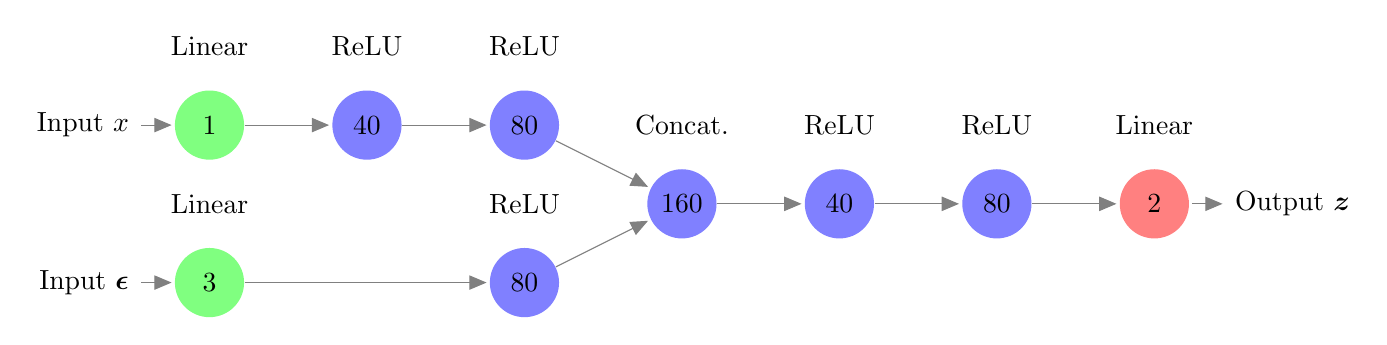
\begin{tikzpicture}[shorten >=1pt,->,draw=black!50, node distance=2.5cm]
    \tikzstyle{every pin edge}=[<-,shorten <=1pt]
    \tikzstyle{neuron}=[circle,fill=black!25,minimum size=25pt,inner sep=0pt]
    \tikzstyle{input neuron}=[neuron, fill=green!50];
    \tikzstyle{output neuron}=[neuron, fill=red!50];
    \tikzstyle{hidden neuron}=[neuron, fill=blue!50];
    \tikzstyle{annot} = [text width=4em, text centered]
    
	%\node[input neuron, pin=left:Bias] (I-0) at (0,0) {$x_0$};
    % Draw the input layer nodes
    %\foreach \name / \y in {1,...,3}
    % This is the same as writing \foreach \name / \y in {1/1,2/2,3/3,4/4}
    \node[input neuron, pin=left:Input $x$] (I-1) at (0,-1) {$1$};
	\node[input neuron, pin=left:Input $\bm{\epsilon}$] (I-2) at (0,-3) {$3$};

    \path[yshift=0cm] node[hidden neuron] (H-11) at (2.0cm,-1) {$40$};
	\path[yshift=0cm] node[hidden neuron] (H-12) at (4.0cm,-1) {$80$};
    \path[yshift=0cm] node[hidden neuron] (H-2) at (4.0cm,-3) {$80$};
    \path[yshift=0cm] node[hidden neuron] (H-3) at (6.0cm,-2) {$160$};
    \path[yshift=0cm] node[hidden neuron] (H-31) at (8.0cm,-2) {$40$};
    \path[yshift=0cm] node[hidden neuron] (H-32) at (10.0cm,-2) {$80$};
	\path[yshift=0cm] node[output neuron,pin={[pin edge={->}]right:Output $\bm{z}$}] (O) at (12.0cm, -2) {$2$};
    \path (I-1) edge (H-11);
    \path (H-11) edge (H-12);
	\path (I-2) edge (H-2);
	\path (H-12) edge (H-3);
	\path (H-2) edge (H-3);
	\path (H-3) edge (H-31);
	\path (H-31) edge (H-32);
	\path (H-32) edge (O);
    % Annotate the layers
    \node[annot,above of=I-1, node distance=1cm] {Linear};
    \node[annot,above of=I-2, node distance=1cm] {Linear};
    \node[annot,above of=H-11, node distance=1cm] {ReLU};
    \node[annot,above of=H-12, node distance=1cm] {ReLU};
    \node[annot,above of=H-2, node distance=1cm] {ReLU};
    \node[annot,above of=H-3, node distance=1cm] {Concat.};
    \node[annot,above of=H-31, node distance=1cm] {ReLU};
    \node[annot,above of=H-32, node distance=1cm] {ReLU};
    \node[annot,above of=O, node distance=1cm] {Linear};
\end{tikzpicture}\\
The number inside the node indicates how many nodes the layer has, and the text above the node describes the activation function in the layer. Recall that the input layer does not have an activation function (Linear), and Rectified Linear Units (ReLU) are used for most of the hidden layers due to their many advantages. In the Concat. layer, the two input vectors are concatenated and there is no activation function placed on the layer. Since arbitrary probability distribution samples can take any real number, we do not use an activation function for the output layer.\\
\\
The structure of the estimator (discriminator $\mathcal{D}_\alpha(z,x)$ or ratio estimator $\mathcal{R}_\alpha(z,x)$) is similar to that of the the generator, with an additional hidden layer associated with the $z$ input and a different activation function for the output layer, corresponding to the estimator's identity. Note that in terms of code, the only differences between class probability estimation and divergence minimisation are the activation function of the estimator's output layer and the loss functions being minimised. A sigmoid output layer is used for a discriminator, whilst a rectified linear output is used for a ratio estimator. The estimator structure is shown in Figure below:\\
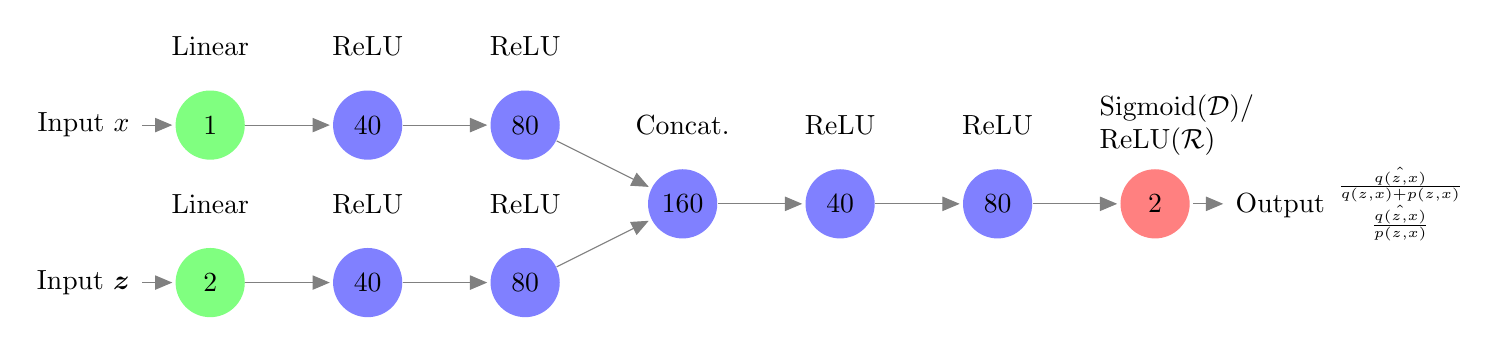
\begin{tikzpicture}[shorten >=1pt,->,draw=black!50, node distance=2.5cm]
    \tikzstyle{every pin edge}=[<-,shorten <=1pt]
    \tikzstyle{neuron}=[circle,fill=black!25,minimum size=25pt,inner sep=0pt]
    \tikzstyle{input neuron}=[neuron, fill=green!50];
    \tikzstyle{output neuron}=[neuron, fill=red!50];
    \tikzstyle{hidden neuron}=[neuron, fill=blue!50];
    \tikzstyle{annot} = [text width=4em, text centered]
    
	%\node[input neuron, pin=left:Bias] (I-0) at (0,0) {$x_0$};
    % Draw the input layer nodes
    %\foreach \name / \y in {1,...,3}
    % This is the same as writing \foreach \name / \y in {1/1,2/2,3/3,4/4}
    \node[input neuron, pin=left:Input $x$] (I-1) at (0,-1) {$1$};
	\node[input neuron, pin=left:Input $\bm{z}$] (I-2) at (0,-3) {$2$};

    \path[yshift=0cm] node[hidden neuron] (H-11) at (2.0cm,-1) {$40$};
	\path[yshift=0cm] node[hidden neuron] (H-12) at (4.0cm,-1) {$80$};
	\path[yshift=0cm] node[hidden neuron] (H-21) at (2.0cm,-3) {$40$};
    \path[yshift=0cm] node[hidden neuron] (H-22) at (4.0cm,-3) {$80$};
    \path[yshift=0cm] node[hidden neuron] (H-3) at (6.0cm,-2) {$160$};
    \path[yshift=0cm] node[hidden neuron] (H-31) at (8.0cm,-2) {$40$};
    \path[yshift=0cm] node[hidden neuron] (H-32) at (10.0cm,-2) {$80$};
	\path[yshift=0cm] node[output neuron,pin={[pin edge={->}]right:Output $\genfrac{}{}{0pt}{}{\hat{\frac{q(z,x)}{q(z,x)+p(z,x)}}}{\hat{\frac{q(z,x)}{p(z,x)}}}$}] (O) at (12.0cm, -2) {$2$};
    \path (I-1) edge (H-11);
    \path (H-11) edge (H-12);
	\path (I-2) edge (H-21);
	\path (H-21) edge (H-22);
	\path (H-12) edge (H-3);
	\path (H-22) edge (H-3);
	\path (H-3) edge (H-31);
	\path (H-31) edge (H-32);
	\path (H-32) edge (O);
    % Annotate the layers
    \node[annot,above of=I-1, node distance=1cm] {Linear};
    \node[annot,above of=I-2, node distance=1cm] {Linear};
    \node[annot,above of=H-11, node distance=1cm] {ReLU};
    \node[annot,above of=H-12, node distance=1cm] {ReLU};
    \node[annot,above of=H-21, node distance=1cm] {ReLU};
    \node[annot,above of=H-22, node distance=1cm] {ReLU};
    \node[annot,above of=H-3, node distance=1cm] {Concat.};
    \node[annot,above of=H-31, node distance=1cm] {ReLU};
    \node[annot,above of=H-32, node distance=1cm] {ReLU};
    \node[annot,above of=O, node distance=1cm] {Sigmoid($\mathcal{D}$)/ ReLU($\mathcal{R}$)};
\end{tikzpicture}\\
The network weights are initialized with Xavier initialization, and trained using the Adam optimizer with learning rate $0.0001$ for the prior-contrastive setting and $0.00001$ for joint-contrastive. Preliminary runs show that these are the highest learning rates at which both algorithms converge consistently; any higher learning rates lead to the program constantly entering a "failure" state (discussed in next section). The network is only trained on the data values $x=0,5,8,12,50$; in each training iteration, 200 samples are taken for each x-value, corresponding to a batch size of 1000. This relatively large batch size makes training more consistent, as performing back-propagation along a stochastic neural network can lead to random and erratic training. To prevent problems associated with taking $\log 0$, we add a small constant $c=10^{-18}$ to the log function's input. The estimator is pre-trained for 5000 iterations to ensure that optimization of the variational network begins with an optimal estimator; an inaccurate ratio estimation leads to incorrect optimization of the posterior network. The variance of the results is also reduced as the initial weights and biases of the estimator will be approximately the same for a fixed initialization of the generator. Afterwards, the generator is optimized for 10000 iterations in the implicit prior formulation, and 40000 iterations when we have an implicit likelihood. The algorithm alternates between 100 training steps of the estimator and 1 training step of the generator. This process for class probability estimation and divergence minimisation is shown in Algorithm and Algorithm below:
\begin{algorithm}
\SetKw{update}{update}
\caption{Sprinkler Prior-Contrastive Class Probability Estimation}
\KwData{Dataset $q^*(x)=\{0,5,8,12,20\}$, true (implicit) prior $p(z)\sim \mathcal{N}(0,2I_{2\times 2})$, true (implicit) likelihood $p(x|z)\sim EXP(3+\max(0,z_1)^3+\max(0,z_2)^3)$, noise distribution $\pi(\epsilon)\sim \mathcal{N}(0,I_{3\times 3})$}
\KwResult{Optimized posterior generator $\mathcal{G}_\phi(\epsilon;x)$}
\BlankLine
\For{$j=1$ \KwTo $5001$}{
	Sample $\{\epsilon^{(i,j)}\}^{1000}_{i=1}\sim \pi(\epsilon)$\;
		Sample $\{0,5,8,12,50\}^{200}_{i=1}=\{x^{(i,j)}\}^{1000}_{i=1}\sim q^*(x)$\;
		Sample $\{z^{(i,j)}_p\}^{1000}_{i=1}\sim p(z)$\;
		\ForEach{$\epsilon^{(i,j)},x^{(i,j)}$}{
			Sample $\{z^{(i,j)}_q\}^{1000}_{i=1}=\mathcal{G}(\epsilon^{(i,j)};x^{(i,j}_q)$\;
		}
		\update{$\alpha$ by optimization step on}{
			$\min_\alpha -\frac{1}{1000}\sum_{i=1}^{1000}\{\log [D_\alpha(\mathcal{G}_\phi(\epsilon^{(i,j)};x^{(i,j)}), x^{(i,j)})]+\log [1-D_\alpha(z_p^{(i,j)},x^{(i,j)})]\}$\;
		}
}
\For{$j=1$ \KwTo $10001$}{
	\For{$k=1$ \KwTo $100$}{	
		Sample $\{\epsilon^{(i,k)}\}^{1000}_{i=1}\sim \pi(\epsilon)$\;
		Sample $\{0,5,8,12,50\}^{200}_{i=1}=\{x^{(i,k)}\}^{1000}_{i=1}\sim q^*(x)$\;
		Sample $\{z^{(i,k)}_p\}^{1000}_{i=1}\sim p(z)$\;
		\ForEach{$\epsilon^{(i,k)},x^{(i,k)}$}{
			Sample $\{z^{(i,k)}_q\}^{1000}_{i=1}=\mathcal{G}(\epsilon^{(i,k)};x^{(i,k)}_q)$\;
		}
		\update{$\alpha$ by optimization step on}{
			$\min_\alpha -\frac{1}{1000}\sum_{i=1}^{1000}\{\log [D_\alpha(\mathcal{G}_\phi(\epsilon^{(i,k)};x^{(i,k)}), x^{(i,k)})]+\log [1-D_\alpha(z_p^{(i,k)},x^{(i,k)})]\}$\;
		}
	}
	Sample $\{\epsilon^{(i)}\}^{1000}_{i=1}\sim \pi(\epsilon)$\;
	Sample $\{0,5,8,12,50\}^{200}_{i=1}=\{x^{(i)}\}^{1000}_{i=1}\sim q^*(x)$\;
	\update{$\phi$ by optimization step on}{
		$\min_\phi \frac{1}{1000}\sum^{1000}_{i=1}\{-\log p(x|\mathcal{G}_\phi(\epsilon^{(i)};x^{(i)}))+\log\frac{D_\alpha(\mathcal{G}_\phi(\epsilon^{(i)};x^{(i)}),x^{(i)})}{1-D_\alpha(\mathcal{G}_\phi(\epsilon^{(i)};x^{(i)}),x^{(i)})}\}$\;
	}
}
\end{algorithm}
\begin{algorithm}
\SetKw{update}{update}
\caption{Sprinkler Prior-Contrastive KL Divergence Minimisation}
\KwData{Dataset $q^*(x)=\{0,5,8,12,20\}$, true (implicit) prior $p(z)\sim \mathcal{N}(0,2I_{2\times 2})$, true (implicit) likelihood $p(x|z)\sim EXP(3+\max(0,z_1)^3+\max(0,z_2)^3)$, noise distribution $\pi(\epsilon)\sim \mathcal{N}(0,I_{3\times 3})$}
\KwResult{Optimized posterior generator $\mathcal{G}_\phi(\epsilon;x)$}
\BlankLine
\For{$j=1$ \KwTo $5001$}{
	Sample $\{\epsilon^{(i,j)}\}^{2000}_{i=1}\sim \pi(\epsilon)$\;
		Sample $\{0,5,8,12,50\}^{400}_{i=1}=\{x^{(i,j)}\}^{2000}_{i=1}\sim q^*(x)$\;
		Sample $\{z^{(i,j)}_p\}^{2000}_{i=1}\sim p(z)$\;
		\ForEach{$\epsilon^{(i,j)},x^{(i,j)}$}{
			Sample $\{z^{(i,j)}_q\}^{2000}_{i=1}=\mathcal{G}(\epsilon^{(i,j)};x^{(i,j})$\;
		}
		\update{$\alpha$ by optimization step on}{
			$\min_\alpha -\frac{1}{2000}\sum_{i=1}^{2000}\{\log [r_\alpha(\mathcal{G}_\phi(\epsilon^{(i,j)};x^{(i,j)}), x^{(i,j)})]+r_\alpha(z_p^{(i,j)},x^{(i,j)})\}$\;
		}
}
\For{$j=1$ \KwTo $10001$}{
	\For{$k=1$ \KwTo $100$}{	
		Sample $\{\epsilon^{(i,k)}\}^{1000}_{i=1}\sim \pi(\epsilon)$\;
		Sample $\{0,5,8,12,50\}^{200}_{i=1}=\{x^{(i,k)}\}^{1000}_{i=1}\sim q^*(x)$\;
		Sample $\{z^{(i,k)}_p\}^{1000}_{i=1}\sim p(z)$\;
		\ForEach{$\epsilon^{(i,k)},x^{(i,k)}$}{
			Sample $\{z^{(i,k)}_q\}^{1000}_{i=1}=\mathcal{G}(\epsilon^{(i,k)};x^{(i,k)}_q)$\;
		}
		\update{$\alpha$ by optimization step on}{
			$\min_\alpha -\frac{1}{1000}\sum_{i=1}^{1000}\{\log [r_\alpha(\mathcal{G}_\phi(\epsilon^{(i,k)};x^{(i,k)}), x^{(i,k)})]+r_\alpha(z_p^{(i,k)},x^{(i,k)})\}$\;
		}
	}
	Sample $\{\epsilon^{(i)}\}^{1000}_{i=1}\sim \pi(\epsilon)$\;
	Sample $\{0,5,8,12,50\}^{200}_{i=1}=\{x^{(i)}\}^{1000}_{i=1}\sim q^*(x)$\;
	\update{$\phi$ by optimization step on}{
		$\min_\phi \frac{1}{1000}\sum^{1000}_{i=1}\{-\log p(x|\mathcal{G}_\phi(\epsilon^{(i)};x^{(i)}))+\log r_\alpha(\mathcal{G}_\phi(\epsilon^{(i)};x^{(i)}),x^{(i)})\}$\;
	}
}
\end{algorithm}
\begin{algorithm}
\SetKw{update}{update}
\caption{Sprinkler Joint-Contrastive Class Probability Estimation}
\KwData{Dataset $q^*(x)=\{0,5,8,12,20\}$, true (implicit) prior $p(z)\sim \mathcal{N}(0,2I_{2\times 2})$, true (implicit) likelihood $p(x|z)\sim EXP(3+\max(0,z_1)^3+\max(0,z_2)^3)$, noise distribution $\pi(\epsilon)\sim \mathcal{N}(0,I_{3\times 3})$}
\KwResult{Optimized posterior generator $\mathcal{G}_\phi(\epsilon;x)$}
\BlankLine
\For{$j=1$ \KwTo $5001$}{
	Sample $\{\epsilon^{(i,j)}\}^{1000}_{i=1}\sim \pi(\epsilon)$\;
		Sample $\{0,5,8,12,50\}^{200}_{i=1}=\{x^{(i,j)}_q\}^{1000}_{i=1}\sim q^*(x)$\;
		Sample $\{z^{(i,j)}_p\}^{1000}_{i=1}\sim p(z)$\;
		\ForEach{$\epsilon^{(i,j)},x^{(i,j)}$}{
			Sample $\{z^{(i,j)}_q\}^{1000}_{i=1}=\mathcal{G}(\epsilon^{(i,j)};x^{(i,j}_q)$\;
		}
		\ForEach{$z^{(i,j)}_p$}{
			Sample $\{x^{(i,j)}_p\}^{1000}_{i=1}\sim p(x|z)$\;
		}
		\update{$\alpha$ by optimization step on}{
			$\min_\alpha -\frac{1}{1000}\sum_{i=1}^{1000}\{\log [D_\alpha(\mathcal{G}_\phi(\epsilon^{(i,j)};x_q^{(i,j)}), x_q^{(i,j)})]+\log [1-D_\alpha(z_p^{(i,j)},x_p^{(i,j)})]\}$\;
		}
}
\For{$j=1$ \KwTo $40001$}{
	\For{$k=1$ \KwTo $100$}{	
		Sample $\{\epsilon^{(i,k)}\}^{1000}_{i=1}\sim \pi(\epsilon)$\;
		Sample $\{0,5,8,12,50\}^{200}_{i=1}=\{x^{(i,k)}_q\}^{1000}_{i=1}\sim q^*(x)$\;
		Sample $\{z^{(i,k)}_p\}^{1000}_{i=1}\sim p(z)$\;
		\ForEach{$\epsilon^{(i,k)},x^{(i,k)}$}{
			Sample $\{z^{(i,k)}_q\}^{1000}_{i=1}=\mathcal{G}(\epsilon^{(i,k)};x^{(i,k)}_q)$\;
		}
		\ForEach{$z^{(i,k)}_p$}{
			Sample $\{x^{(i,k)}_p\}^{1000}_{i=1}\sim p(x|z)$\;
		}
		\update{$\alpha$ by optimization step on}{
			$\min_\alpha -\frac{1}{1000}\sum_{i=1}^{1000}\{\log [D_\alpha(\mathcal{G}_\phi(\epsilon^{(i,k)};x_q^{(i,k)}), x_q^{(i,k)})]+\log [1-D_\alpha(z_p^{(i,k)},x_p^{(i,k)})]\}$\;
		}
	}
	Sample $\{\epsilon^{(i)}\}^{1000}_{i=1}\sim \pi(\epsilon)$\;
	Sample $\{0,5,8,12,50\}^{200}_{i=1}=\{x^{(i)}_q\}^{1000}_{i=1}\sim q^*(x)$\;
	\update{$\phi$ by optimization step on}{
		$\min_\phi \frac{1}{1000}\sum^{1000}_{i=1}\log\frac{D_\alpha(\mathcal{G}_\phi(\epsilon^{(i)};x_q^{(i)}),x_q^{(i)})}{1-D_\alpha(\mathcal{G}_\phi(\epsilon^{(i)};x_q^{(i)}),x_q^{(i)})}$\;
	}
}
\end{algorithm}
\begin{algorithm}
\SetKw{update}{update}
\caption{Sprinkler Joint-Contrastive KL Divergence Minimisation}
\KwData{Dataset $q^*(x)=\{0,5,8,12,20\}$, true (implicit) prior $p(z)\sim \mathcal{N}(0,2I_{2\times 2})$, true (implicit) likelihood $p(x|z)\sim EXP(3+\max(0,z_1)^3+\max(0,z_2)^3)$, noise distribution $\pi(\epsilon)\sim \mathcal{N}(0,I_{3\times 3})$}
\KwResult{Optimized posterior generator $\mathcal{G}_\phi(\epsilon;x)$}
\BlankLine
\For{$j=1$ \KwTo $5001$}{
	Sample $\{\epsilon^{(i,j)}\}^{1000}_{i=1}\sim \pi(\epsilon)$\;
		Sample $\{0,5,8,12,50\}^{200}_{i=1}=\{x^{(i,j)}_q\}^{1000}_{i=1}\sim q^*(x)$\;
		Sample $\{z^{(i,j)}_p\}^{1000}_{i=1}\sim p(z)$\;
		\ForEach{$\epsilon^{(i,j)},x^{(i,j)}$}{
			Sample $\{z^{(i,j)}_q\}^{1000}_{i=1}=\mathcal{G}(\epsilon^{(i,j)};x^{(i,j}_q)$\;
		}
		\ForEach{$z^{(i,j)}_p$}{
			Sample $\{x^{(i,j)}_p\}^{1000}_{i=1}\sim p(x|z)$\;
		}
		\update{$\alpha$ by optimization step on}{
			$\min_\alpha -\frac{1}{1000}\sum_{i=1}^{1000}\{\log [r_\alpha(\mathcal{G}_\phi(\epsilon^{(i,j)};x_q^{(i,j)}), x_q^{(i,j)})]+r_\alpha(z_p^{(i,j)},x_p^{(i,j)})\}$\;
		}
}
\For{$j=1$ \KwTo $40001$}{
	\For{$k=1$ \KwTo $100$}{	
		Sample $\{\epsilon^{(i,k)}\}^{1000}_{i=1}\sim \pi(\epsilon)$\;
		Sample $\{0,5,8,12,50\}^{200}_{i=1}=\{x^{(i,k)}_q\}^{1000}_{i=1}\sim q^*(x)$\;
		Sample $\{z^{(i,k)}_p\}^{1000}_{i=1}\sim p(z)$\;
		\ForEach{$\epsilon^{(i,k)},x^{(i,k)}$}{
			Sample $\{z^{(i,k)}_q\}^{1000}_{i=1}=\mathcal{G}(\epsilon^{(i,k)};x^{(i,k)}_q)$\;
		}
		\ForEach{$z^{(i,k)}_p$}{
			Sample $\{x^{(i,k)}_p\}^{1000}_{i=1}\sim p(x|z)$\;
		}
		\update{$\alpha$ by optimization step on}{
			$\min_\alpha -\frac{1}{1000}\sum_{i=1}^{1000}\{\log [r_\alpha(\mathcal{G}_\phi(\epsilon^{(i,k)};x_q^{(i,k)}), x_q^{(i,k)})]+r_\alpha(z_p^{(i,k)},x_p^{(i,k)})\}$\;
		}
	}
	Sample $\{\epsilon^{(i)}\}^{1000}_{i=1}\sim \pi(\epsilon)$\;
	Sample $\{0,5,8,12,50\}^{200}_{i=1}=\{x^{(i)}_q\}^{1000}_{i=1}\sim q^*(x)$\;
	\update{$\phi$ by optimization step on}{
		$\min_\phi \frac{1}{1000}\sum^{1000}_{i=1}\log r_\alpha(\mathcal{G}_\phi(\epsilon^{(i)};x_q^{(i)}),x_q^{(i)})$\;
	}
}
\end{algorithm}
\newpage
\section{Results}
We evaluate the techniques by comparing the average KL divergence between the true and variational posterior distributions at the end of the program's runtime: $\E_{q^*(x)}KL(q(z|x)||p(z|x)) = \E_{q^*(x)}\E_{q(z|x)}\log \frac{q(z|x)}{p(z|x)}$. We do not use the ELBO output of the program to calculate this KL divergence, nor do we compare the ELBOs of the algorithms, as the accuracy of the ELBO estimator is dependent on the algorithm used. Instead, we use a non-parametric approach, estimating the probability density function of the variational posterior output with a Gaussian kernel density estimator $\hat{q}(z|x)$. By using five kernel density estimators for the five data points, we are able to create an estimate of the average KL divergence with an accuracy that is independent of the algorithm used: $\E_{q^*(x)}KL(\hat{q}(z|x)||p(z|x)) = \E_{q^*(x)}\E_{q(z|x)}\log \frac{\hat{q}(z|x)}{p(z|x)}$. Each algorithm was run 30 times and the estimator losses and NELBO estimations for each iteration was stored. Every 100 iterations, kernel density estimation was used to estimate the average KL divergence. The arrays storing the three recorded values were averaged over the 30 repetitions, to enforce reliable experimentation.\\
Clearly, the prior-contrastive algorithms converged much faster their joint-contrastive equivalent, as expected since knowledge of the likelihood improves posterior optimization. Overall, for both PC and JC, we found that class probability estimation performed consistently better than KL divergence minimisation. The means and standard deviations of the results can be found in Table, and it can be seen that the KL minimisation approach had higher average KL divergence and standard deviation, implying that the method is slower and more inconsistent. The estimator loss, estimated NELBO and 'true' KL Divergence over the iterations can be found in Figures. The inconsistency of KL minimisation can be seen in the wild fluctuations early in the estimator loss and NELBO graphs, implying that the NELBO is being estimated inaccurately. This corresponds to the instances in the true KL Divergence graphs where the posterior output worsens over certain periods. Each iteration took approximately the same amount of time to compute (0.32 seconds on me PC), as the bulk of the training time is spent training the neural networks, which have similar structures.\\
Furthermore, in approximately half of the simulations, the ratio loss of the KL divergence minimisation algorithm would start at a relatively high number (42.3 as opposed to 3.5), and it would be stuck there for the entire runtime of the program; the thousands of iterations spent minimizing the ratio loss did not decrease it. At higher training rates, the KL minimization algorithm would sometimes enter this "failure" stage during the main optimization stage. The high ratio loss signifies a very inaccurate ratio estimator, leading to a completely inaccurate variational posterior (i have a fig to isnert here). Thus, the program was programmed to restart every time the ratio loss initialized at a high number, until a reasonable value was initialized. 
\newpage
\chapter{Theory Crafting}
In an attempt to explain why class probability estimation is significantly superior to KL minimization, we compare the two techniques in terms of their 'lower bound' formulation, and analyze their fundamental differences.
\section{Introduction}
For both the prior-contrastive and joint-contrastive formulations, it can be seen that the only differences between CPE and KL min are the function that is optimized to formulate the density ratio estimator, and the parametrization of the estimator. Recall that optimization of the estimator for the KL min algorithm follows the lower bound:
\[D_{KL}(p||q)\geq \sup_{\alpha}\{\mathbb{E}_{q(u)}[1+\log r_\alpha(u)]-\mathbb{E}_{p(u)}[r_\alpha(u)]\}\]
with equality at $r_\alpha(u)=\frac{q(u)}{p(u)}$ and that optimization for class probability estimation follows:
\[2D_{JS}(p||q)-\log 4\geq \sup_\alpha\{\mathbb{E}_{q(u)}[\log \mathcal{D}_\alpha(u)]+\mathbb{E}_{p(u)}[\log(1-\mathcal{D}_\alpha(u))]\}\]
with equality at $D_\alpha(u)=\frac{q(u)}{q(u)+p(u)}$.\\
These two estimators can be used interchangeably, as $D_\alpha(u)=\frac{r_\alpha(u)}{r_\alpha(u)+1}$ and $r_\alpha(u)=\frac{D_\alpha(u)}{1-D_\alpha(u)}$. In fact, the former transformation is used to derive this formulation of the discriminative loss for class probability estimation. By transforming the estimators used in the two f-divergences, we can formulate two new estimator optimization problems:
\[\min_\alpha \mathbb{E}_{q(u)}[\log D_\alpha (u)-\log(1-D_\alpha(u))]-\mathbb{E}_{p(u)}\frac{D_\alpha(u)}{1-D_\alpha(u)}\]
and
\[\min_\alpha -\mathbb{E}_{q(u)}[\log r_\alpha(u)-\log (r_\alpha(u)+1)]+\mathbb{E}_{p(u)}[\log(r_\alpha(u)+1)].\]
The optimization problem for the ELBO in both prior-contrastive and joint-contrastive methods involves density ratio estimation between the true and variational distributions, and the optimization of the likelihood term in the prior-contrastive method is independent of the ratio estimator. We can therefore denote the two ELBO optimization problems for the two estimator parametrizations $D_\alpha (u)$ and $r_\alpha(u)$ as:
\[\min_\phi \mathbb{E}_{q_\phi(u)}\log \frac{D_\alpha (u)}{1-D_\alpha (u)}\quad(+\text{ Likelihood})\]
and
\[\min_\phi \mathbb{E}_{q_\phi(u)}\log r_\alpha (u)\quad(+\text{ Likelihood}).\]
Additionally, we can parametrize the estimator such that it estimates the log ratio directly: $T_\alpha(u)=\log r_\alpha(u)$. This simplifies the objective function for our variational neural network weights to:
\[\min_\phi -\mathbb{E}_{q_\phi(u)}[T_\alpha(u)]\quad(+\text{ Likelihood}).\]
For the KL Divergence, the estimator is optimized as follows:
\[\min_\alpha -\mathbb{E}_{q(u)}[T_\alpha(u)]+\mathbb{E}_{p(u)}[e^{T_\alpha (u)}]\]
The CPE divergence equivalent is:
\[\min_\alpha -\E_{q(u)}\left[\log \frac{e^{T_\alpha(u)}}{e^{T_\alpha(u)}+1}\right]+\E_{p(u)}[\log(e^{T_\alpha(u)}+1)]\]
\section{Recap because its confusing}
To recap, we have mathematically simplified the choice of algorithm for training ratio estimators for implicit variational neural networks to a choice of f-divergence:
\begin{itemize}
\item KL Divergence: $D_{KL}(p||q)=\mathbb{E}_{q(u)}[1+\log \frac{q(u)}{p(u)}]-\mathbb{E}_{p(u)}\left[\frac{q(u)}{p(u)}\right]$
\item CPE Divergence: $D_{CPE}(p||q)=\mathbb{E}_{q(u)}\left[\log \frac{q(u)}{q(u)+p(u)}\right]+\mathbb{E}_{p(u)}\left[\log \frac{p(u)}{q(u)+p(u)}\right]$
\end{itemize}
and a choice of estimator parametrization:
\begin{itemize}
\item Direct ratio estimator: $r^*_\alpha(u)=\frac{q(u)}{p(u)}$
\item "Class probability" estimator: $D^*_\alpha(u)=\frac{q(u)}{q(u)+p(u)}$
\item Direct log ratio estimator: $T^*_\alpha(u)=\log \frac{q(u)}{p(u)}$
\end{itemize}
The original "KL minimization approach" simply chooses the KL Divergence and the direct ratio estimator, and "Class probability estimation" uses the CPE Divergence and the "Class probability" estimator. These are just 2 variations of the 6 available algorithms.
\section{First and Second Derivatives of all 6 possible algorithms}
To evaluate the effectiveness of gradient descent optimization in these algorithms, we formulate the first and second derivatives of the objective functions. We first take the "Class probability" parametrization and observe its optimization problem for the CPE divergence:
\begin{align*}
f_{CPE}(u)&=-\E_{q(u)}[\log D(u)]-\E_{p(u)}[\log (1-D(u))]\\
&=-\int_u q(u)\log D(u) du -\int_u p(u)\log(1-D)du\\
\frac{df}{dD(u)}&=-\frac{q(u)}{D(u)}+\frac{p(u)}{1-D(u)}\\
\frac{d^2f}{dD^2(u)}&=\frac{q(u)}{D^2(u)}+\frac{p(u)}{(1-D(u))^2}\\
&>0 \quad \forall q(u)\in(0,1), p(u)\in (0,1), D(u)\in (0,1) 
\end{align*}
Since the second derivative is always greater than zero, the function is strictly convex and therefore converges linearly with gradient descent.\\
Now observe the optimization problem for the KL Divergence:
\begin{align*}
f_{KL}(u)&=-\E_{q(u)}\left(\log \frac{D(u)}{1-D(u)}\right)+\E_{p(u)}\left(\frac{D(u)}{1-D(u)}\right)\\
&=-\int_u q(u)\left(\log \frac{D(u)}{1-D(u)}\right)du+\int_u p(u)\left(\frac{D(u)}{1-D(u)}\right)du\\
\frac{df}{dD(u)}&=-\frac{q(u)}{D(u)}-\frac{q(u)}{1-D(u)}+\frac{p(u)}{1-D(u)}+\frac{p(u)D(u)}{(1-D(u))^2}\\
&=-\frac{q(u)}{D(u)}-\frac{q(u)}{1-D(u)}+\frac{p(u)}{(1-D(u))^2}\\
\frac{d^2f}{dD^2(u)}&=\frac{q(u)}{D^2(u)}-\frac{q(u)}{(1-D(u))^2}+\frac{2p(u)}{(1-D(u))^3}
\end{align*}
CPE with ratio parametrisation:
\begin{align*}
f_{CPE}(u)&=-\E_{q(u)}\left[\log \frac{r(u)}{r(u)+1}\right]+\E_{p(u)}\left[\log(r(u)+1)\right]\\
&=-\int_u q(u)\left[\log \frac{r(u)}{r(u)+1}\right]du+\int_u p(u)\left[\log(r(u)+1)\right]du\\
\frac{df}{dr(u)}&=-\frac{q(u)}{r(u)}+\frac{q(u)}{r(u)+1}+\frac{p(u)}{r(u)+1}\\
\frac{d^2f}{dr^2(u)}&=\frac{q(u)}{r^2(u)}-\frac{q(u)}{(r(u)+1)^2}-\frac{p(u)}{(r(u)+1)^2}
\end{align*}
KL with ratio parametrisation:
\begin{align*}
f_{KL}(u)&=-\E_{q(u)}(\log r(u))+\E_{p(u)}r\\
&=-\int_u q(u)\log r(u) du+\int_u p(u)r(u)du\\
\frac{df}{dr(u)}&=-\frac{q(u)}{r(u)}+p(u)\\
\frac{d^2f}{dr^2(u)}&=\frac{q(u)}{r^2(u)}\\
&>0
\end{align*}
CPE with log ratio parametrisation:
\begin{align*}
f_{CPE}(u)&=-\E_{q(u)}[T(u)-\log(e^{T(u)}+1)]+\E_{p(u)}[\log(e^{T(u)}+1)]\\
&=\int_u q(u)[\log(e^{T(u)}+1)-T(u)] du+\int_u p(u)[\log(e^{T(u)}+1)]du\\
\frac{df}{dT(u)}&=-q(u)+\frac{(q(u)+p(u))e^{T(u)}}{e^{T(u)}+1}\\
\frac{d^2f}{dT^2(u)}&=\frac{(q(u)+p(u))\exp(T(u))}{e^{T(u)}+1}-\frac{(q(u)+p(u))e^{2T(u)}}{(e^{T(u)}+1)^2}\\
&=\frac{(q(u)+p(u))(e^{2T(u)}+e^{T(u)})-(q(u)+p(u))e^{2T(u)}}{(e^{T(u)}+1)^2}\\
&=\frac{(q(u)+p(u))e^{T(u)}}{(e^{T(u)}+1)^2}\\
&>0
\end{align*}
KL with log ratio parametrisation:
\begin{align*}
f_{KL}(u)&=-\E_{q(u)}[T(u)]+\E_{p(u)}[e^{T(u)}]\\
&=-\int_u q(u)T(u)du+\int_u p(u)e^{T(u)}du\\
\frac{df}{dT(u)}&=-q(u)+p(u)e^{T(u)}\\
\frac{d^2f}{dT^2(u)}&=p(u)e^{T(u)}\\
&>0
\end{align*}
\section{Difference between divergences}
Recall that both divergences attain the same global minimum, which is a parametrization of the estimator, and that these estimators are optimized via stochastic gradient descent. Thus, for a fixed estimator parametrization, the divergences will have varying rates of convergence, which can be analyzed by observing the second derivative. The convergence rate of a gradient descent method is proportional to the size of its second derivative. Due to the variable nature of $p(u)$, $q(u)$ and $D(u)$/$r(u)$/$T(u)$, it is uncertain whether a divergence is superior in this aspect when its second derivative is not strictly greater than the other divergence's equivalent. We are therefore unable to arrive at a certain conclusion for the "Class probability" and direct log ratio estimators, but it can be seen that in the direct ratio parametrisation, the KL divergence is strictly greater than the CPE divergence, implying that it would be superior. However, due to the significant number of iterations taken for each estimator optimization step, it is unlikely the different divergences have a significant impact on the quality of the method. This can be additionally seen in the non-significant decrease in estimator loss over the later half of its optimization step.\\
The effectiveness of different divergences has also been tested in (Nowozin, 2016). They found that the ideal f-divergence used for the estimator's loss function is the same f-divergence that is being minimized in the variational posterior training: in this case, it is the KL divergence. This provides support for our theory that the KL divergence is superior (at least in the direct ratio case).
\section{Difference between estimators}
Again, we compare the second derivatives of the techniques, this time fixing the divergence and observing the difference in estimator parametrization. Due to the exponential term in the log ratio parametrisation, no conclusion can be drawn from its comparisons. We cannot conclude anything from comparing the remaining two estimators for the KL divergence either. It can however be seen that for the CPE divergence, the "Class probability" parametrization is strictly superior.\\
Now consider the bounds on the estimators. The class probability estimator with an optimal form of $\frac{q(u)}{q(u)+p(u)}$ is bound in $(0,1)$, so from any arbitrary starting point in the same space, very few optimization steps are required to reach the global minimum. On the other hand, the direct ratio estimator is bound in $\R^+ \ \{0\}$, and the direct log ratio estimator can take any value in $\R$, so optimization can take many iterations if the difference between the estimator's initial and optimal values is too large. This can be problematic if there are insufficient iterations of optimizing the estimator, particularly in the initialization stage: the estimator may not properly converge and the posterior will be trained with an inaccurate density ratio estimation.\\
Furthermore, we can also consider the effect of the posterior density displacement from each training step: every time $q_\phi(u)$ changes, the optimal value of the estimator also changes. Consequently, the estimator must take optimization steps to 'catch up', but again, if the displacement is too significant, then the estimator may not converge in time. From the bounds, it is intuitive that the class probability estimator's global minimum displaces less than the direct ratio estimator. It can also be shown that $|D^*_{final}-D^*_{init}|<|r^*_{final}-r^*_{init}|$:\\
Letting $\epsilon\neq0$ be the change in $q(u)$ with an optimization step, and noting that $|\epsilon|<q(u)$, we have
\begin{align*}
|D^*_{final}-D^*_{init}|&=\left|\frac{q(u)+\epsilon}{q(u)+\epsilon+p(u)}-\frac{q(u)}{q(u)+p(u)}\right|\\
&=\left|\frac{q^2(u)+q(u)p(u)+\epsilon q(u)+\epsilon p(u)}{(q(u)+\epsilon+p(u))(q(u)+p(u))}-\frac{q^2(u)+\epsilon q(u)+q(u)p(u)}{(q(u)+\epsilon+p(u))(q(u)+p(u))}\right|\\
&=\left|\frac{\epsilon p(u)}{(q(u)+\epsilon+p(u))(q(u)+p(u))}\right|\\
&=\left|\frac{\epsilon}{(q(u)+\epsilon+p(u))(\frac{q(u)}{p(u)}+1)}\right|\\
|r^*_{final}-r^*_{init}|&=\left|\frac{q(u)+\epsilon}{p(u)}-\frac{q(u)}{p(u)}\right|\\
&=\left|\frac{\epsilon}{p(u)}\right|\\
\end{align*}
If $\epsilon>0$, then
\[|D^*_{final}-D^*_{init}|<|r^*_{final}-r^*_{init}|\text{ as }(q(u)+\epsilon+p(u))(\frac{q(u)}{p(u)}+1)>p(u).\]
If $\epsilon<0$, then recalling that $|\epsilon| < q(u) < q(u)+p(u)$,
\begin{align*}
(q(u)+\epsilon+p(u))(\frac{q(u)}{p(u)}+1)&=\frac{q^2(u)}{p(u)}+2q(u)+p(u)+\epsilon \left(\frac{q(u)}{p(u)}+1\right)\\
&=(q(u)+\epsilon)\left(\frac{q(u)}{p(u)}+1\right)+q(u)+p(u)\\
&>p(u)
\end{align*}
For the direct log ratio estimator, we have
\begin{align*}
|T^*_{final}-T^*_{init}|&=\left|\log \frac{q(u)+\epsilon}{p(u)}-\log \frac{q(u)}{p(u)}\right|\\
&=\left|\log \frac{q(u)+\epsilon}{q(u)}\right|
\end{align*}
It is difficult to make a direct comparison with the other displacement expressions.\\
We now address the "failures" experienced by the KL minimization algorithm. Consider that the activation function of the estimator network's output layer, influencing the output range, varies between the estimators. For the direct ratio estimator, ReLU is used for the output, meaning that a 0 is outputted if the previous matrix operations lead to a negative number. Now recall that we take the log of the ratio estimator's output in all of the related optimization problems, and that a small constant $c$ is added to prevent taking the log of $0$. This explains the 'failures' of the KL minimization algorithm: the neural network has been initialised such that a $0$ is outputted, signifying that the previous matrix operations led to a negative number. Its loss function takes a large value according to this scenario (e.g. for KL minimization, it is $-\log c$), and does not decrease over training iterations, as a slight change in the network weights would still output the same result, meaning that the partial derivative of the weights with respect to the loss function is $0$. Due to this occurrence, the "failures" would additionally occur in the direct log ratio estimator, as its output layer is simply the log of a ReLU output, which would suffer from the same problem. On the other hand, the sigmoid activation function of the "Class probability" estimator is bound in $(0,1)$, so it does not experience any "failures".\\
Aside from the failures, the difference in output activation functions could also explain our experimental results; the rectified linear unit models the density ratio in a linear manner, meaning that it would be asymmetric, in the sense that cases where $q(u)>p(u)$ result in any output in $(1,\infty)$, but if $p(u)<q(u)$, then the outputted is limited to $(0,1)$. On the other hand, the sigmoid function has symmetric output, as if $q(u)>p(u)$, it is bound in $(0.5,1)$, and if $q(u)<p(u)$, the outputs lie within $(0,0.5)$. Taking the log of the rectified linear output and optimizing the objective functions with respect to it may partially resolve this issue, as the cases will become bound in $(0,\infty)$ and $(-\infty,0)$ respectively, but it would retain an additional issue: having a rectified linear unit for the output layer restricts the previous matrix operations to have an output in $\R^{+}\backslash \{0\}$, as its surjective mapping truncates $\R^-$. On the other hand, the sigmoid output layer has a bijective mapping from $\R$ to $(0,1)$.\\
Instead of using the naive ReLU activation function, we propose to use an exponential activation function for the direct ratio estimator, and a linear activation function for the log ratio estimator. The exponential function is even and bijective, mapping $\R^-$ to $(0,1)$ and $\R^+$ to $(1,\infty)$. Similarly, the linear activation keeps the output in $\R$, which is the space of the log ratio estimator. We believe that this will resolve the key issues in our KL minimization approach: the estimator outputs will be more consistent throughout the early training period and there will be no failures caused by an output of $0$.
\chapter{Inference Experiments - "Sprinkler"}
\section{Determining optimal activation function}
\subsection{Experiment Outline}
Since we have identified two possible representations for both the direct density ratio and log density ratio estimations, we first compare them to find the ideal activation function. Additionally, if our proposed activation functions prevent the "failures" from occurring, then the posterior training rate can be increased for the following experiments, reducing the computational time required to complete them. The experiment setup is exactly the same as the previous experiment, with the same repetitions, training rates and iterations, but we now aim to compare the ReLU and exponential activation functions for direct density ratio estimation, as well as the log ReLU and linear activation functions for direct log density ratio estimation. These comparisons will be made in four different contexts: both the CPE and KL divergences will be used in both of the prior-contrastive and joint-contrastive environments.
\subsection{Results}
Firstly, we note that the bijective activation functions did not experience any failures. This alone confirms our theory as to why the failures occur, and that the surjective activation functions are inferior for this particular purpose. Comparing the simulations that haven't failed, we have the following tables and figures showing the results. It can be seen that the means and standard deviations of the true KL divergence are consistently lower for the exponential and linear activation functions. This is due to the lack of fluctuations in their estimator losses and NELBO estimations, supporting our theory that the unevenness of the ReLU activation function correlates to inconsistent training and outputs.
\newpage
\section{Comparing Estimator Accuracies}
\subsection{Experiment Outline}
Now that we have identified optimal activation functions for the estimators, we now verify that the estimators, when optimally trained, lead to similar levels of convergence, regardless of the divergence used or the estimator parametrisation. Again, the setup is the same as in the previous two experiments, with low training rates and high iterations to ensure smooth posterior convergence and optimality of the estimator. Note that at this point, we already have experimental results for all of the divergence and estimator combinations except for the KL divergence with class probability estimator. Thus, to save computational time, we reuse those results.
\subsection{Results}
From the figures below, we can see that for each divergence, the graphs of the three estimators are indistinguishable. The final KL divergences in the table below also shows no significant difference between the divergences or estimator parametrizations used. The key point of this result is that it does not matter which estimator training combination is used as long as it is optimally trained.
\newpage
\section{Comparing Accuracies of Undertrained Estimators}
\subsection{Experiment Outline}
In this experiment, we aim to confirm our theory that the estimators only differ when improperly trained, and that an estimator's accuracy directly correlates with its training rate. We therefore significantly reduce the amount of estimator training between each posterior iteration, lowering the estimator training rate to 0.00004 and the estimator steps to 15 in the prior-contrastive setting, and 20 for the joint-contrastive algorithm. We also increase the posterior training rate to 0.0002 and to account for this change, the number of optimization steps of the variational distribution was reduced to 2000 for prior-contrastive and 4000 for joint-contrastive. The other training parameters were kept consistent with the previous experiments.
\subsection{Results}
From the table, it can be seen that the class probability estimator is superior to the direct ratio estimator, which is better than the log ratio estimator. This is supportive of our theories detailing the estimator output bounds, displacements and second derivatives as factors affecting training speed. The theory of second derivatives, as well as Nowozin's paper is further supported by the superiority of the KL divergence. It is difficult to discern any related trends in the figures: most of the estimator and NELBO plots have wild fluctuations at the start of the training period, which settles down to a steady decline at about the same point for all three estimators. Most interesting is the joint-contrastive CPE divergence plots for estimator loss and NELBO, which demonstrates greater fluctuations of the direct ratio estimator, deviating from the other two estimators. Despite this, the estimator's effectiveness lies between the other two estimators. This trend is not experienced by any of the other contexts either.
\newpage
\chapter{Data Generation - (MNIST image generation)}
\section{Problem Context}
The MNIST (Modified National Institute of Standards and Technology) dataset is widely used for testing machine learning algorithms related to image analysis. It contains 60,000 training and 10,000 testing images of handwritten digits, each grayscale and of 28x28 pixel size. Thus, the image distribution has 784 dimensions and follows a Bernoulli distribution. A sample of the images can be seen in Figure.\\
In this problem, we aim to generate new MNIST images indistinguishable from those in the original dataset. To do so, we use the algorithm described in section, alternating between density ratio estimator training and simultaneous training of an encoder that maps images to a lower dimensional normal distribution and a decoder that generates new images using samples from the same latent space.\\
Recall that joint-contrastive algorithms are more suited to pairing between different sample spaces than for data generation, so we only formulate prior-contrastive algorithms for this experiment. The main goal of this experiment is to compare the estimator parametrizations for high dimensional data, verifying the result from the last Sprinkler experiment. We repeat the experiment with two different latent spaces, one with 2 dimensions and one with 10 dimensions, to determine if the dimensionality of the densities in the density ratio $\frac{q_\phi(z|x)}{p(z)}$ has any effect.
\section{Program Structure}
Both our posterior sample generator and estimator have the same structures as in the Sprinkler problem, except the number of posterior noise inputs and nodes per layer have increased to account for the higher dimensionality of the problem. Although this problem involves image analysis, due to its simplicity we refrain from using convolutional layers, similar to other experiments (insert ref). To model the problem's likelihood function, we use an additional decoder network that is trained simultaneously with the posterior. Its structure is as shown in Figure below:\\
A training rate of 0.0004 is used for all of the optimization steps, with a batch size of 512. Again, the estimator is pre-trained for 5000 iterations, afterwards the program alternates between 20 iterations of estimator optimizaton and 1 iteration of posterior training, for 4000 total posterior iterations.
\section{Results}
The higher dimensional problem shows an estimator that is clearly superior. In this part of the experiment, the values involved with estimating the direct density ratio and log density ratio are greater than the largest positive number representable by a 64-bit floating point number, and the program overflows to Inf. This occurs during the estimator initialization phase when the KL divergence between the two distributions is the greatest. The class probability estimator is the only estimator that does not experience this problem.\\
This is because the density ratio $\frac{q_\phi(z|x)}{p(z)}$ increases exponentially with the dimensionality of the latent space, eventually reaching a value that is too large to be represented by a computer. For both direct density ratio algorithms, the estimator network is programmed to output $\E_{p(z)q^*(x)}\frac{q_\phi(z|x)}{p(z)}$ directly, and if the log density ratio is estimated instead, its exponential is taken in the estimator loss function, leading back to the direct density ratio. On the other hand, the class probability estimator output is bound in $(0,1)$, so a large density ratio would cause the estimate to output a number near 1. In fact, since the sigmoid activation function is used to map the network output from $R$ to $(0,1)$, it can be easily shown that the input of the activation function is the log ratio (we can output this value directly, slightly reducing the computation time needed to calculate the log ratio in this parametrization). Letting $x$ be the neural network output before being mapped to $(0,1)$, we have:
\begin{align*}
\frac{1}{1+e^{-x}}&=\frac{q_\phi(z|x)}{p(z)+q_\phi(z|x)}\\
e^{-x}+1&=\frac{p(z)+q_\phi(z|x)}{q_\phi(z|x)}\\
e^{-x}&=\frac{p(z)}{q_\phi(z|x)}\\
x&=\log \frac{q_\phi(z|x)}{p(z)}.
\end{align*}
The calculations involved with the class probability estimator are therefore within the space of representable number by 64-bit, and even 32-bit floating point numbers. Using a 32-bit representation leads to much faster computations. We can therefore conclude that the class probability estimator is superior in the sense that it is the only feasible parametrization.
\chapter{Related Work and Discussion}
Leave this as a brainstorm list for now
\begin{itemize}
\item Of course many other problems and training parameters can be explored, variational inference and implicit models are used for more than inference and generation
\item More f-divergences can be explored (Nowozin, 2016)
\item Could test estimators for CycleGANs (joint-contrastive formulation for images) (Tiao, 2018)
\item Could take a step back from using neural networks to estimate the divergence, instead try divergence estimation via k-nearest-neighbour distances (Wang, 2009)
\item I don't know how denoisers work but they may be comparable to the methods discussed in this thesis (Huszar)
\item Hopefully in the future everyone will be using class probability estimators trained under the loss function formulated by the KL divergence :)
\end{itemize}
\chapter{Conclusion}
This thesis is hot trash.





%%%%%%%%%%%%%%%%%%%%%%%%%%%%%%%%%%%%%%%%%%%%%%%%%%%%%%%%%%%%%%%%%%%%%%%%%%
\clearpage
\addcontentsline{toc}{chapter}{References}
\bibliographystyle{apalike}
\bibliography{bible}



\newpage
\appendix
\chapter{Kernel Density Estimation}
Kernel density estimation is a non-parametric method used to estimate the probability density function of a distribution, using only samples. It can therefore be used to estimate implicit distributions. For simplicity we only explain the univariate form of the kernel density estimator, though the multivariate form is used in this thesis.

Let $\{x^{(i)}\}^n_{i=1}$ be an independent and identically distributed sample from a distribution with unknown probability density function $f$. Its kernel density estimator is defined as
\[\hat{f}_h(x)=\frac{1}{nh}\sum^n_{i=1}K\left(\frac{x-x^{(i)}}{h}\right).\]
$K$ is the kernel, a symmetric non-negative weighting function that integrates to 1. Examples of kernel functions are:
\begin{itemize}
\item Epanechnikov: $K(u)=\frac{3}{4}(1-u^2), |u|\leq 1$
\item Uniform: $K(u)=\frac12, |u|\leq 1$
\item Gaussian: $K(u)=\frac{1}{\sqrt{2\pi}}\exp\left(-\frac{1}{2}u^2\right)$.
\end{itemize}
Typically, the Gaussian kernel is used due to its statistical properties, but the choice of kernel is not as important as the choice of $h$, the bandwidth.

The bandwidth $h>0$ acts as a smoothing parameter, determining the width of the kernel. If $h$ is too small, $\hat{f}$ will be 'undersmoothed' as too much weight is placed on the areas nearest the data-points, leading to a spiky estimate with high variance. On the other hand, if $h$ is too large, $\hat{f}$ will be 'oversmoothed' with too little weight on areas nearest to the data-points, resulting in a relatively flat estimate with high bias. It is therefore ideal to choose $h$ such that the mean integrated square error $MISE(h)=\E\left[\int(\hat{f}_h(x)-f(x))^2dx\right]$ is minimized. For a Gaussian kernel, this is approximately $h=1.06\hat{\sigma}n^{-1/5}$ where $\hat{\sigma}$ is the sample standard deviation. We omit the proof in this thesis.

The kernel density estimator works by placing a kernel on each data point and summing up the kernels to produce a smooth curve. Each point on the curve is essentially a weighted average of nearby data points. Regions of the curve with many data points will therefore have a high estimated probability density.
\end{document}





